% Options for packages loaded elsewhere
\PassOptionsToPackage{unicode}{hyperref}
\PassOptionsToPackage{hyphens}{url}
%
\documentclass[
]{article}
\usepackage{amsmath,amssymb}
\usepackage{iftex}
\ifPDFTeX
  \usepackage[T1]{fontenc}
  \usepackage[utf8]{inputenc}
  \usepackage{textcomp} % provide euro and other symbols
\else % if luatex or xetex
  \usepackage{unicode-math} % this also loads fontspec
  \defaultfontfeatures{Scale=MatchLowercase}
  \defaultfontfeatures[\rmfamily]{Ligatures=TeX,Scale=1}
\fi
\usepackage{lmodern}
\ifPDFTeX\else
  % xetex/luatex font selection
\fi
% Use upquote if available, for straight quotes in verbatim environments
\IfFileExists{upquote.sty}{\usepackage{upquote}}{}
\IfFileExists{microtype.sty}{% use microtype if available
  \usepackage[]{microtype}
  \UseMicrotypeSet[protrusion]{basicmath} % disable protrusion for tt fonts
}{}
\makeatletter
\@ifundefined{KOMAClassName}{% if non-KOMA class
  \IfFileExists{parskip.sty}{%
    \usepackage{parskip}
  }{% else
    \setlength{\parindent}{0pt}
    \setlength{\parskip}{6pt plus 2pt minus 1pt}}
}{% if KOMA class
  \KOMAoptions{parskip=half}}
\makeatother
\usepackage{xcolor}
\usepackage[margin=1in]{geometry}
\usepackage{color}
\usepackage{fancyvrb}
\newcommand{\VerbBar}{|}
\newcommand{\VERB}{\Verb[commandchars=\\\{\}]}
\DefineVerbatimEnvironment{Highlighting}{Verbatim}{commandchars=\\\{\}}
% Add ',fontsize=\small' for more characters per line
\usepackage{framed}
\definecolor{shadecolor}{RGB}{248,248,248}
\newenvironment{Shaded}{\begin{snugshade}}{\end{snugshade}}
\newcommand{\AlertTok}[1]{\textcolor[rgb]{0.94,0.16,0.16}{#1}}
\newcommand{\AnnotationTok}[1]{\textcolor[rgb]{0.56,0.35,0.01}{\textbf{\textit{#1}}}}
\newcommand{\AttributeTok}[1]{\textcolor[rgb]{0.13,0.29,0.53}{#1}}
\newcommand{\BaseNTok}[1]{\textcolor[rgb]{0.00,0.00,0.81}{#1}}
\newcommand{\BuiltInTok}[1]{#1}
\newcommand{\CharTok}[1]{\textcolor[rgb]{0.31,0.60,0.02}{#1}}
\newcommand{\CommentTok}[1]{\textcolor[rgb]{0.56,0.35,0.01}{\textit{#1}}}
\newcommand{\CommentVarTok}[1]{\textcolor[rgb]{0.56,0.35,0.01}{\textbf{\textit{#1}}}}
\newcommand{\ConstantTok}[1]{\textcolor[rgb]{0.56,0.35,0.01}{#1}}
\newcommand{\ControlFlowTok}[1]{\textcolor[rgb]{0.13,0.29,0.53}{\textbf{#1}}}
\newcommand{\DataTypeTok}[1]{\textcolor[rgb]{0.13,0.29,0.53}{#1}}
\newcommand{\DecValTok}[1]{\textcolor[rgb]{0.00,0.00,0.81}{#1}}
\newcommand{\DocumentationTok}[1]{\textcolor[rgb]{0.56,0.35,0.01}{\textbf{\textit{#1}}}}
\newcommand{\ErrorTok}[1]{\textcolor[rgb]{0.64,0.00,0.00}{\textbf{#1}}}
\newcommand{\ExtensionTok}[1]{#1}
\newcommand{\FloatTok}[1]{\textcolor[rgb]{0.00,0.00,0.81}{#1}}
\newcommand{\FunctionTok}[1]{\textcolor[rgb]{0.13,0.29,0.53}{\textbf{#1}}}
\newcommand{\ImportTok}[1]{#1}
\newcommand{\InformationTok}[1]{\textcolor[rgb]{0.56,0.35,0.01}{\textbf{\textit{#1}}}}
\newcommand{\KeywordTok}[1]{\textcolor[rgb]{0.13,0.29,0.53}{\textbf{#1}}}
\newcommand{\NormalTok}[1]{#1}
\newcommand{\OperatorTok}[1]{\textcolor[rgb]{0.81,0.36,0.00}{\textbf{#1}}}
\newcommand{\OtherTok}[1]{\textcolor[rgb]{0.56,0.35,0.01}{#1}}
\newcommand{\PreprocessorTok}[1]{\textcolor[rgb]{0.56,0.35,0.01}{\textit{#1}}}
\newcommand{\RegionMarkerTok}[1]{#1}
\newcommand{\SpecialCharTok}[1]{\textcolor[rgb]{0.81,0.36,0.00}{\textbf{#1}}}
\newcommand{\SpecialStringTok}[1]{\textcolor[rgb]{0.31,0.60,0.02}{#1}}
\newcommand{\StringTok}[1]{\textcolor[rgb]{0.31,0.60,0.02}{#1}}
\newcommand{\VariableTok}[1]{\textcolor[rgb]{0.00,0.00,0.00}{#1}}
\newcommand{\VerbatimStringTok}[1]{\textcolor[rgb]{0.31,0.60,0.02}{#1}}
\newcommand{\WarningTok}[1]{\textcolor[rgb]{0.56,0.35,0.01}{\textbf{\textit{#1}}}}
\usepackage{longtable,booktabs,array}
\usepackage{calc} % for calculating minipage widths
% Correct order of tables after \paragraph or \subparagraph
\usepackage{etoolbox}
\makeatletter
\patchcmd\longtable{\par}{\if@noskipsec\mbox{}\fi\par}{}{}
\makeatother
% Allow footnotes in longtable head/foot
\IfFileExists{footnotehyper.sty}{\usepackage{footnotehyper}}{\usepackage{footnote}}
\makesavenoteenv{longtable}
\usepackage{graphicx}
\makeatletter
\def\maxwidth{\ifdim\Gin@nat@width>\linewidth\linewidth\else\Gin@nat@width\fi}
\def\maxheight{\ifdim\Gin@nat@height>\textheight\textheight\else\Gin@nat@height\fi}
\makeatother
% Scale images if necessary, so that they will not overflow the page
% margins by default, and it is still possible to overwrite the defaults
% using explicit options in \includegraphics[width, height, ...]{}
\setkeys{Gin}{width=\maxwidth,height=\maxheight,keepaspectratio}
% Set default figure placement to htbp
\makeatletter
\def\fps@figure{htbp}
\makeatother
\setlength{\emergencystretch}{3em} % prevent overfull lines
\providecommand{\tightlist}{%
  \setlength{\itemsep}{0pt}\setlength{\parskip}{0pt}}
\setcounter{secnumdepth}{-\maxdimen} % remove section numbering
\ifLuaTeX
  \usepackage{selnolig}  % disable illegal ligatures
\fi
\usepackage{bookmark}
\IfFileExists{xurl.sty}{\usepackage{xurl}}{} % add URL line breaks if available
\urlstyle{same}
\hypersetup{
  pdftitle={Machine Learning Computer Lab 1 Block2 (Group A7)},
  pdfauthor={Qinyuan Qi(qinqi464); Satya Sai Naga Jaya Koushik Pilla (satpi345); Daniele Bozzoli(danbo826)},
  hidelinks,
  pdfcreator={LaTeX via pandoc}}

\title{Machine Learning Computer Lab 1 Block2 (Group A7)}
\author{Qinyuan Qi(qinqi464) \and Satya Sai Naga Jaya Koushik Pilla
(satpi345) \and Daniele Bozzoli(danbo826)}
\date{2024-01-10}

\begin{document}
\maketitle

\subsection{Assignment 1: KERNEL METHODS(Solved by Qinyuan
Qi)}\label{assignment-1-kernel-methodssolved-by-qinyuan-qi}

\subsubsection{Answer:}\label{answer}

In this assignment, we will try to predict the temp of Linköping station
on date 1970-11-05.

The 3 basic kernel functions are implemented as follows.

\begin{Shaded}
\begin{Highlighting}[]
\DocumentationTok{\#\#\#\#\#\#\#\#\#\#\#\#\#\#\#\#\#\#\#\#\#\#\#\#\# Kernel Code  \#\#\#\#\#\#\#\#\#\#\#\#\#\#\#\#\#\#\#\#\#\#\#\#\#\#\#\#\#\#\#\#\#\#\#\#\#}
\CommentTok{\# Gaussian kernel of geo distance}
\NormalTok{geo\_distance }\OtherTok{\textless{}{-}} \ControlFlowTok{function}\NormalTok{(data, location\_interest, h\_dist) \{}
\NormalTok{  location }\OtherTok{\textless{}{-}} \FunctionTok{data.frame}\NormalTok{(}\AttributeTok{longitude =}\NormalTok{ data}\SpecialCharTok{$}\NormalTok{longitude,}
                         \AttributeTok{latitude  =}\NormalTok{ data}\SpecialCharTok{$}\NormalTok{latitude)}
\NormalTok{  distances }\OtherTok{\textless{}{-}} \FunctionTok{distHaversine}\NormalTok{(location\_interest,location)}
\NormalTok{  kernel\_result }\OtherTok{\textless{}{-}} \FunctionTok{exp}\NormalTok{(}\SpecialCharTok{{-}}\NormalTok{(distances)}\SpecialCharTok{\^{}}\DecValTok{2} \SpecialCharTok{/}\NormalTok{ (}\DecValTok{2} \SpecialCharTok{*}\NormalTok{ h\_dist}\SpecialCharTok{\^{}}\DecValTok{2}\NormalTok{))}
  \FunctionTok{return}\NormalTok{(}\FunctionTok{c}\NormalTok{(distances, kernel\_result))}
\NormalTok{\}}

\CommentTok{\# Gaussian kernel of day distance}
\NormalTok{day\_distance }\OtherTok{\textless{}{-}} \ControlFlowTok{function}\NormalTok{(data, day\_interest, h\_day) \{}
\NormalTok{  distances }\OtherTok{\textless{}{-}} \FunctionTok{as.numeric}\NormalTok{(}\FunctionTok{difftime}\NormalTok{(day\_interest,data, }
                          \AttributeTok{units =} \StringTok{"days"}\NormalTok{))}
\NormalTok{  kernel\_result }\OtherTok{\textless{}{-}} \FunctionTok{exp}\NormalTok{(}\SpecialCharTok{{-}}\NormalTok{(distances)}\SpecialCharTok{\^{}}\DecValTok{2} \SpecialCharTok{/}\NormalTok{ (}\DecValTok{2} \SpecialCharTok{*}\NormalTok{ h\_day}\SpecialCharTok{\^{}}\DecValTok{2}\NormalTok{))}
  \FunctionTok{return}\NormalTok{(}\FunctionTok{c}\NormalTok{(distances, kernel\_result))}
\NormalTok{\}}

\CommentTok{\# Gaussian kernel of hour distance}
\NormalTok{hour\_distance }\OtherTok{\textless{}{-}} \ControlFlowTok{function}\NormalTok{(data, hour\_interest, h\_hour) \{}
  
\NormalTok{  diff }\OtherTok{\textless{}{-}} \FunctionTok{sapply}\NormalTok{(}\DecValTok{1}\SpecialCharTok{:}\FunctionTok{length}\NormalTok{(hour\_interest), }\ControlFlowTok{function}\NormalTok{(x)\{}
              \FunctionTok{abs}\NormalTok{(}\FunctionTok{as.numeric}\NormalTok{(}\FunctionTok{difftime}\NormalTok{(}\FunctionTok{strptime}\NormalTok{(hour\_interest[x], }\StringTok{"\%H:\%M:\%S"}\NormalTok{), }
                                      \FunctionTok{strptime}\NormalTok{(data}\SpecialCharTok{$}\NormalTok{time, }\StringTok{"\%H:\%M:\%S"}\NormalTok{)), }\AttributeTok{units=}\StringTok{"hours"}\NormalTok{))}
\NormalTok{  \})}
  
\NormalTok{  distances }\OtherTok{\textless{}{-}} \FunctionTok{ifelse}\NormalTok{(diff }\SpecialCharTok{\textless{}=} \DecValTok{12}\NormalTok{, diff, }\DecValTok{24}\SpecialCharTok{{-}}\NormalTok{diff)}
\NormalTok{  kernel\_result }\OtherTok{\textless{}{-}} \FunctionTok{exp}\NormalTok{(}\SpecialCharTok{{-}}\NormalTok{(distances)}\SpecialCharTok{\^{}}\DecValTok{2} \SpecialCharTok{/}\NormalTok{ (}\DecValTok{2} \SpecialCharTok{*}\NormalTok{ h\_day}\SpecialCharTok{\^{}}\DecValTok{2}\NormalTok{))}
  \FunctionTok{return}\NormalTok{(kernel\_result)}
\NormalTok{\}}
\end{Highlighting}
\end{Shaded}

We set h\_distance=100000, and set station to Linköping, then we plot
the kernel function for distance as follows.

\begin{Shaded}
\begin{Highlighting}[]
\DocumentationTok{\#\#\#\#\#\#\#\#\#\#\#\#\#\#\#\#\#\#\#\#\#\#\#\#\#\#\#\#\#\#\#\# 1.1 Distance Kernel \#\#\#\#\#\#\#\#\#\#\#\#\#\#\#\#\#\#\#\#\#\#\#\#\#\#\#}

\CommentTok{\# These three values are up to the students}
\NormalTok{h\_distance }\OtherTok{\textless{}{-}} \DecValTok{100000}

\CommentTok{\# set coordinates to predict(Linköping)}
\NormalTok{a }\OtherTok{\textless{}{-}}\NormalTok{ stations}\SpecialCharTok{$}\NormalTok{longitude[station\_row]}
\NormalTok{b }\OtherTok{\textless{}{-}}\NormalTok{ stations}\SpecialCharTok{$}\NormalTok{latitude[station\_row]}

\NormalTok{N }\OtherTok{\textless{}{-}} \FunctionTok{nrow}\NormalTok{(train)}
\NormalTok{i }\OtherTok{\textless{}{-}} \DecValTok{1}\SpecialCharTok{:}\NormalTok{N}
\NormalTok{k\_distance }\OtherTok{\textless{}{-}} \FunctionTok{sapply}\NormalTok{(i, }\ControlFlowTok{function}\NormalTok{(i)\{}\FunctionTok{geo\_distance}\NormalTok{(train[i, ], }\FunctionTok{c}\NormalTok{(a, b), h\_distance)\})}
\FunctionTok{plot}\NormalTok{(k\_distance[}\DecValTok{1}\NormalTok{,], k\_distance[}\DecValTok{2}\NormalTok{,], }\AttributeTok{main =} \StringTok{"Distance Gaussian Kernel"}\NormalTok{, }\AttributeTok{xlab =} \StringTok{"Distance"}\NormalTok{, }\AttributeTok{ylab =} \StringTok{"K"}\NormalTok{)}
\end{Highlighting}
\end{Shaded}

\includegraphics{Lab3_files/figure-latex/1.1-1.pdf}

We set h\_day=20, then we plot the kernel function as follows.

\begin{Shaded}
\begin{Highlighting}[]
\DocumentationTok{\#\#\#\#\#\#\#\#\#\#\#\#\#\#\#\#\#\#\#\#\#\#\#\#\#\#\#\#\#\#\#\# 1.2 Day Kernel \#\#\#\#\#\#\#\#\#\#\#\#\#\#\#\#\#\#\#\#\#\#\#\#\#\#\#\#\#\#\#}
\NormalTok{h\_day }\OtherTok{\textless{}{-}} \DecValTok{20}
\NormalTok{k\_day }\OtherTok{\textless{}{-}} \FunctionTok{sapply}\NormalTok{(i, }\ControlFlowTok{function}\NormalTok{(i) }\FunctionTok{day\_distance}\NormalTok{(}\FunctionTok{as.Date}\NormalTok{(train}\SpecialCharTok{$}\NormalTok{date[i]), date\_interest, h\_day))}
\FunctionTok{plot}\NormalTok{(k\_day[}\DecValTok{1}\NormalTok{,], k\_day[}\DecValTok{2}\NormalTok{,], }\AttributeTok{main =} \StringTok{"Day Gaussian Kernel"}\NormalTok{, }\AttributeTok{xlab =} \StringTok{"Days"}\NormalTok{, }\AttributeTok{ylab =} \StringTok{"K"}\NormalTok{)}
\end{Highlighting}
\end{Shaded}

\includegraphics{Lab3_files/figure-latex/1.2-1.pdf}

We set h\_hour = 7.

\begin{Shaded}
\begin{Highlighting}[]
\DocumentationTok{\#\#\#\#\#\#\#\#\#\#\#\#\#\#\#\#\#\#\#\#\#\#\#\#\#\#\#\#\#\#\#\# 1.3 Hour Kernel \#\#\#\#\#\#\#\#\#\#\#\#\#\#\#\#\#\#\#\#\#\#\#\#\#\#\#\#\#\#\#}

\NormalTok{h\_hour }\OtherTok{\textless{}{-}} \DecValTok{7}

\CommentTok{\# Get the time format we want}
\NormalTok{times\_interest }\OtherTok{\textless{}{-}} \FunctionTok{c}\NormalTok{(}\FunctionTok{paste0}\NormalTok{(}\StringTok{"0"}\NormalTok{,}\FunctionTok{seq}\NormalTok{(}\DecValTok{4}\NormalTok{,}\DecValTok{8}\NormalTok{,}\AttributeTok{by=}\DecValTok{2}\NormalTok{),}\StringTok{":00:00"}\NormalTok{), }\FunctionTok{paste0}\NormalTok{(}\FunctionTok{seq}\NormalTok{(}\DecValTok{10}\NormalTok{,}\DecValTok{24}\NormalTok{,}\AttributeTok{by=}\DecValTok{2}\NormalTok{),}\StringTok{":00:00"}\NormalTok{))}

\NormalTok{k\_hour }\OtherTok{\textless{}{-}} \FunctionTok{sapply}\NormalTok{(i, }\ControlFlowTok{function}\NormalTok{(i) }\FunctionTok{hour\_distance}\NormalTok{(train[i,], times\_interest, h\_hour))}
\end{Highlighting}
\end{Shaded}

Now we setting up another new kernel(sum of 3 kernels), and plot the
prediction value as follows.

\begin{Shaded}
\begin{Highlighting}[]
\DocumentationTok{\#\#\#\#\#\#\#\#\#\#\#\#\#\#\#\#\#\#\#\#\#\#\#\#\#\#\#\#\#\#\#\# 1.4 Sum Kernel \#\#\#\#\#\#\#\#\#\#\#\#\#\#\#\#\#\#\#\#\#\#\#\#\#\#\#\#\#\#\#}
\NormalTok{predicted\_temp\_sum }\OtherTok{\textless{}{-}} \FunctionTok{sapply}\NormalTok{(}\DecValTok{1}\SpecialCharTok{:}\FunctionTok{length}\NormalTok{(times\_interest), }\ControlFlowTok{function}\NormalTok{(x) }
        \FunctionTok{sum}\NormalTok{((k\_distance[}\DecValTok{2}\NormalTok{,] }\SpecialCharTok{+}\NormalTok{ k\_day[}\DecValTok{2}\NormalTok{,] }\SpecialCharTok{+}\NormalTok{ k\_hour[x,]) }\SpecialCharTok{*}\NormalTok{ train}\SpecialCharTok{$}\NormalTok{air\_temperature)}
        \SpecialCharTok{/} \FunctionTok{sum}\NormalTok{(k\_distance[}\DecValTok{2}\NormalTok{,], k\_day[}\DecValTok{2}\NormalTok{,], k\_hour[x,]))}

\FunctionTok{plot}\NormalTok{(}\FunctionTok{seq}\NormalTok{(}\DecValTok{4}\NormalTok{,}\DecValTok{24}\NormalTok{,}\AttributeTok{by=}\DecValTok{2}\NormalTok{),predicted\_temp\_sum, }\AttributeTok{type=}\StringTok{"l"}\NormalTok{, }
\AttributeTok{main =} \StringTok{"Temp in Linkoping(Sum)"}\NormalTok{, }\AttributeTok{xlab =} \StringTok{"Time"}\NormalTok{, }\AttributeTok{ylab =} \StringTok{"Temp"}\NormalTok{)}
\end{Highlighting}
\end{Shaded}

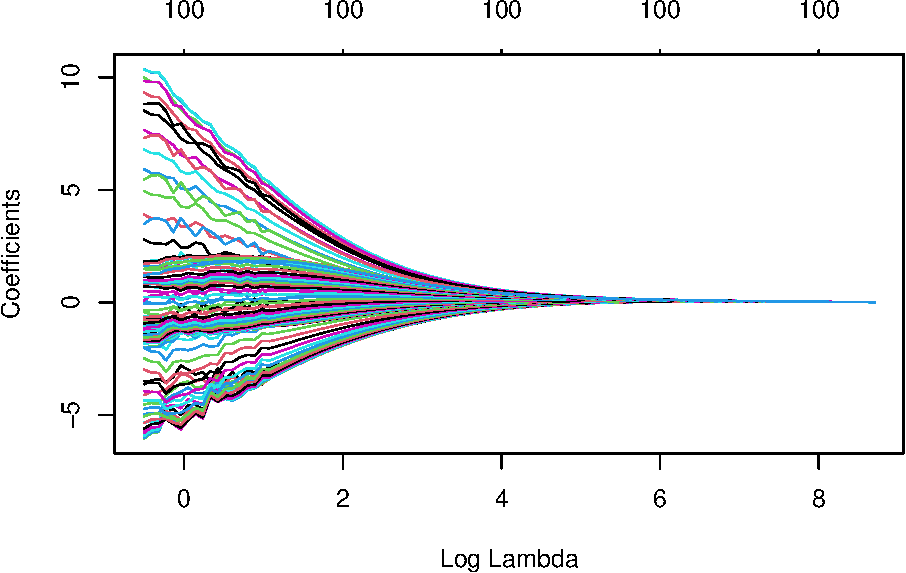
\includegraphics{Lab3_files/figure-latex/1.4-1.pdf}

Now we setting up another new kernel(mul of 3 kernels), and plot the
prediction value as follows.

\begin{Shaded}
\begin{Highlighting}[]
\DocumentationTok{\#\#\#\#\#\#\#\#\#\#\#\#\#\#\#\#\#\#\#\#\#\#\#\#\#\#\#\#\#\#\#\# 1.5 Multi Kernel \#\#\#\#\#\#\#\#\#\#\#\#\#\#\#\#\#\#\#\#\#\#\#\#\#\#\#\#\#\#\#}
\NormalTok{predicted\_temp\_mul }\OtherTok{\textless{}{-}} \FunctionTok{sapply}\NormalTok{(}\DecValTok{1}\SpecialCharTok{:}\FunctionTok{length}\NormalTok{(times\_interest), }\ControlFlowTok{function}\NormalTok{(x) }
        \FunctionTok{sum}\NormalTok{((k\_distance[}\DecValTok{2}\NormalTok{,] }\SpecialCharTok{*}\NormalTok{ k\_day[}\DecValTok{2}\NormalTok{,] }\SpecialCharTok{*}\NormalTok{ k\_hour[x,]) }\SpecialCharTok{*}\NormalTok{ train}\SpecialCharTok{$}\NormalTok{air\_temperature)}
        \SpecialCharTok{/} \FunctionTok{sum}\NormalTok{(k\_distance[}\DecValTok{2}\NormalTok{,] }\SpecialCharTok{*}\NormalTok{ k\_day[}\DecValTok{2}\NormalTok{,] }\SpecialCharTok{*}\NormalTok{ k\_hour[x,]))}

\FunctionTok{plot}\NormalTok{(}\FunctionTok{seq}\NormalTok{(}\DecValTok{4}\NormalTok{,}\DecValTok{24}\NormalTok{,}\AttributeTok{by=}\DecValTok{2}\NormalTok{),predicted\_temp\_mul, }\AttributeTok{type=}\StringTok{"l"}\NormalTok{, }
\AttributeTok{main =} \StringTok{"Temp in Linkoping (Mul)"}\NormalTok{, }\AttributeTok{xlab =} \StringTok{"Time"}\NormalTok{, }\AttributeTok{ylab =} \StringTok{"Temp"}\NormalTok{)}
\end{Highlighting}
\end{Shaded}

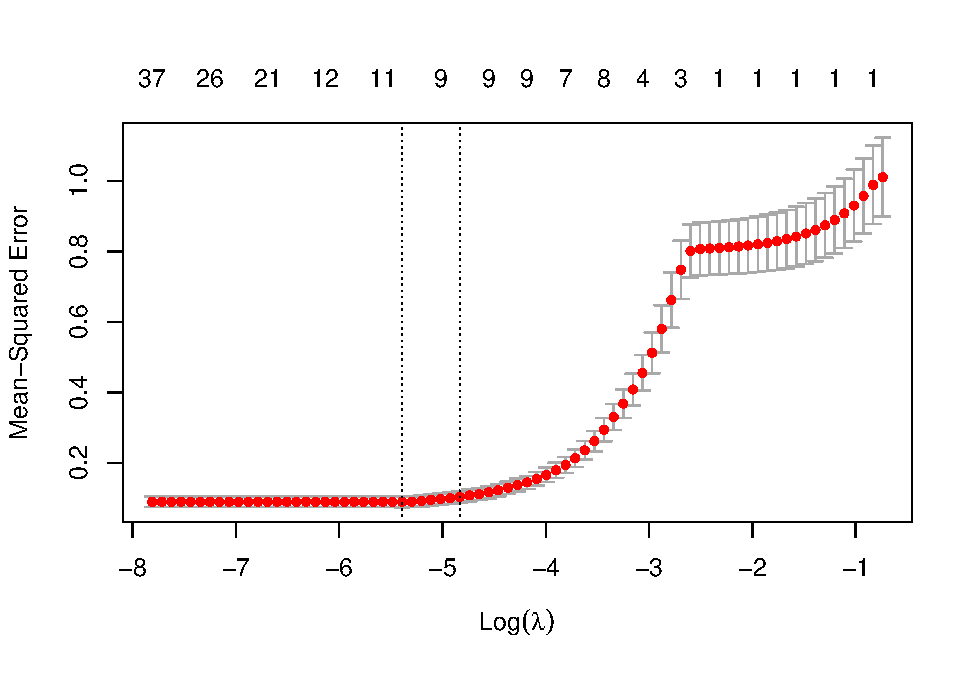
\includegraphics{Lab3_files/figure-latex/1.5-1.pdf} Compare the sum and
mul version of the kernel, we can see that there have around 1 degree
difference. According to the real results, we found the following near
Nov in Linköping.

1962-10-09,18:00:00,9.6 / 1971-11-29,06:00:00,0 / 1975-11-06,12:00:00,10
/ 1961-11-02,18:00:00,11

It seems that the predictions still have some gaps near the real
results.

\subsection{Assignment 2: SUPPORT VECTOR MACHINES(Solved by Satya Sai
Naga Jaya Koushik
Pilla)}\label{assignment-2-support-vector-machinessolved-by-satya-sai-naga-jaya-koushik-pilla}

\subsubsection{Answer:}\label{answer-1}

According to the code, we know that the spam data is splitted into
training,validation,training+validation, and test data respectively.

According to the code output, we know that the minimal error is 0.0675
when C = 0.3.

\begin{verbatim}
## minimal error = 0.0675  when C = 3.9
\end{verbatim}

Also we draw the plot of error\_va versus C as follows.

\includegraphics{Lab3_files/figure-latex/2.1.2-1.pdf}

\subsubsection{2.1. Which filter do we return to the user ? filter0,
filter1, filter2 or filter3?
Why?}\label{which-filter-do-we-return-to-the-user-filter0-filter1-filter2-or-filter3-why}

Then we calc the error rate of 4 filters, accoring to this, we know the
accuracy rates are as follows.

\begin{longtable}[]{@{}ccc@{}}
\toprule\noalign{}
Filter & Accuracy & Accept / Reject \\
\midrule\noalign{}
\endhead
\bottomrule\noalign{}
\endlastfoot
filter0 & 93.25 \% & Accept \\
\end{longtable}

Filter0 follow the best practice and get the highest accuracy rate. It
train on training data,it predict on validation data

\begin{longtable}[]{@{}ccc@{}}
\toprule\noalign{}
Filter & Accuracy & Accept / Reject \\
\midrule\noalign{}
\endhead
\bottomrule\noalign{}
\endlastfoot
filter1 & 91.51061 \% & Reject \\
\end{longtable}

Filter1 follow the best practice but its accuracy rate is lower than
filter 0. It train on training data,it predict on test data

\begin{longtable}[]{@{}ccc@{}}
\toprule\noalign{}
Filter & Accuracy & Accept / Reject \\
\midrule\noalign{}
\endhead
\bottomrule\noalign{}
\endlastfoot
filter2 & 91.7603 \% & Reject \\
\end{longtable}

Filter2 does not follow the best practice but still practiciable, It
train on training+validation data, predict on test data, also its
accuracy rate is lower than filter 0.

\begin{longtable}[]{@{}ccc@{}}
\toprule\noalign{}
Filter & Accuracy & Accept / Reject \\
\midrule\noalign{}
\endhead
\bottomrule\noalign{}
\endlastfoot
filter3 & 97.87765 \% & Reject \\
\end{longtable}

Filter3 training on all data,and using the seen data to predict which is
not accepetable.

Based on the analysis above, we should return filter0 to the user.

\subsubsection{2.2 What is the estimate of the generalization error of
the filter returned to the user? err0, err1, err2 or err3?
Why?}\label{what-is-the-estimate-of-the-generalization-error-of-the-filter-returned-to-the-user-err0-err1-err2-or-err3-why}

Generalization error is the expectation of the the predicted values of
an independent test set on our model.

Based on the test data, we got the following result.

The reason why filter0 and filter1 are same is because these 2 filters
share the same parameters and are same.

\begin{verbatim}
## generalization error of filter0 is 8.489388 %
\end{verbatim}

\begin{verbatim}
## generalization error of filter1 is 8.489388 %
\end{verbatim}

\begin{verbatim}
## generalization error of filter2 is 8.2397 %
\end{verbatim}

\begin{verbatim}
## generalization error of filter3 is 2.122347 %
\end{verbatim}

\subsubsection{2.3 Implementation of SVM
predictions.}\label{implementation-of-svm-predictions.}

The missing code implemented as follows.

\begin{Shaded}
\begin{Highlighting}[]
\NormalTok{sv }\OtherTok{\textless{}{-}} \FunctionTok{alphaindex}\NormalTok{(filter3)[[}\DecValTok{1}\NormalTok{]]}
\NormalTok{co}\OtherTok{\textless{}{-}}\FunctionTok{coef}\NormalTok{(filter3)[[}\DecValTok{1}\NormalTok{]]}
\NormalTok{inte}\OtherTok{\textless{}{-}} \SpecialCharTok{{-}} \FunctionTok{b}\NormalTok{(filter3)}
\CommentTok{\# RBF kernel with sigma = 0.05}
\NormalTok{rbf }\OtherTok{\textless{}{-}} \FunctionTok{rbfdot}\NormalTok{(}\AttributeTok{sigma =} \FloatTok{0.05}\NormalTok{) }
\NormalTok{k}\OtherTok{\textless{}{-}}\ConstantTok{NULL}
\CommentTok{\# We produce predictions for just the first 10 points in the dataset.}
\ControlFlowTok{for}\NormalTok{(i }\ControlFlowTok{in} \DecValTok{1}\SpecialCharTok{:}\DecValTok{10}\NormalTok{)\{ }
\NormalTok{  k2}\OtherTok{\textless{}{-}}\ConstantTok{NULL}
  \ControlFlowTok{for}\NormalTok{(j }\ControlFlowTok{in} \DecValTok{1}\SpecialCharTok{:}\FunctionTok{length}\NormalTok{(sv))\{}
\NormalTok{    k2 }\OtherTok{\textless{}{-}}\NormalTok{ k2 }\SpecialCharTok{+}\NormalTok{ co[j] }\SpecialCharTok{*} \FunctionTok{rbf}\NormalTok{(}\FunctionTok{as.numeric}\NormalTok{(spam[sv[j], }\SpecialCharTok{{-}}\DecValTok{58}\NormalTok{]),}
                           \FunctionTok{as.numeric}\NormalTok{(spam[i, }\SpecialCharTok{{-}}\DecValTok{58}\NormalTok{]))}
\NormalTok{  \}}
\NormalTok{  k}\OtherTok{\textless{}{-}}\FunctionTok{c}\NormalTok{(k,  k2 }\SpecialCharTok{+}\NormalTok{ inte)}
\NormalTok{\}}
\NormalTok{k}
\end{Highlighting}
\end{Shaded}

\begin{verbatim}
## numeric(0)
\end{verbatim}

\begin{Shaded}
\begin{Highlighting}[]
\NormalTok{pred\_filter3 }\OtherTok{\textless{}{-}} \FunctionTok{predict}\NormalTok{(filter3,spam[}\DecValTok{1}\SpecialCharTok{:}\DecValTok{10}\NormalTok{,}\SpecialCharTok{{-}}\DecValTok{58}\NormalTok{], }\AttributeTok{type =} \StringTok{"decision"}\NormalTok{)}
\NormalTok{pred\_filter3}
\end{Highlighting}
\end{Shaded}

\begin{verbatim}
##            [,1]
##  [1,] -1.998999
##  [2,]  1.560584
##  [3,]  1.000278
##  [4,] -1.756815
##  [5,] -2.669577
##  [6,]  1.291312
##  [7,] -1.068444
##  [8,] -1.312493
##  [9,]  1.000184
## [10,] -2.208639
\end{verbatim}

\subsection{Assignment 3: NEURAL NETWORKS(Solved by Daniele
Bozzoli)}\label{assignment-3-neural-networkssolved-by-daniele-bozzoli}

\subsubsection{Answer:}\label{answer-2}

\subsubsection{3.1}\label{section}

We observe in the plot that the predictions using neural network seem to
be good predictions for the sine function.

Since this function is differentiable, it will also provide a smooth
gradient.

\begin{Shaded}
\begin{Highlighting}[]
\DocumentationTok{\#\#\#\#\#\#\#\#\#\#\#\#\#\#\#\#\#\#\#\#\#\#\#\#\#\#\#  3.1 \#\#\#\#\#\#\#\#\#\#\#\#\#\#\#\#\#\#\#\#\#\#\#\#\#\#\#\#\#\#\#\#\#\#\#\#\#\#\#\#\#\#\#\#\#\#\#\#}
\NormalTok{rand\_var }\OtherTok{\textless{}{-}} \FunctionTok{runif}\NormalTok{(}\DecValTok{500}\NormalTok{, }\DecValTok{0}\NormalTok{, }\DecValTok{10}\NormalTok{)}
\NormalTok{df }\OtherTok{\textless{}{-}} \FunctionTok{data.frame}\NormalTok{(rand\_var, }\AttributeTok{Sin=}\FunctionTok{sin}\NormalTok{(rand\_var))}
\NormalTok{train }\OtherTok{\textless{}{-}}\NormalTok{ df[}\DecValTok{1}\SpecialCharTok{:}\DecValTok{25}\NormalTok{,] }\CommentTok{\# Training}
\NormalTok{test }\OtherTok{\textless{}{-}}\NormalTok{ df[}\DecValTok{26}\SpecialCharTok{:}\DecValTok{500}\NormalTok{,] }\CommentTok{\# Test}

\CommentTok{\# Random initialization of the weights in the interval [{-}1, 1]}
\NormalTok{winit }\OtherTok{\textless{}{-}} \FunctionTok{runif}\NormalTok{(}\DecValTok{31}\NormalTok{, }\SpecialCharTok{{-}}\DecValTok{1}\NormalTok{, }\DecValTok{1}\NormalTok{)}
\NormalTok{nn }\OtherTok{\textless{}{-}} \FunctionTok{neuralnet}\NormalTok{(}\AttributeTok{data =}\NormalTok{ train, }\AttributeTok{formula =}\NormalTok{ Sin }\SpecialCharTok{\textasciitilde{}}\NormalTok{ rand\_var, }\AttributeTok{hidden =} \FunctionTok{c}\NormalTok{(}\DecValTok{10}\NormalTok{))}

\CommentTok{\# Plot of the training data (black), test data (blue), and predictions (red)}
\FunctionTok{plot}\NormalTok{(train,  }\AttributeTok{col =} \StringTok{"black"}\NormalTok{, }\AttributeTok{cex=}\DecValTok{1}\NormalTok{, }\AttributeTok{main=}\StringTok{"Default"}\NormalTok{)}
\FunctionTok{points}\NormalTok{(test, }\AttributeTok{col =} \StringTok{"blue"}\NormalTok{, }\AttributeTok{cex=}\DecValTok{1}\NormalTok{)}
\FunctionTok{points}\NormalTok{(test[,}\DecValTok{1}\NormalTok{], }\FunctionTok{predict}\NormalTok{(nn,test), }\AttributeTok{col=}\StringTok{"red"}\NormalTok{, }\AttributeTok{cex=}\DecValTok{1}\NormalTok{)}
\FunctionTok{legend}\NormalTok{(}\AttributeTok{x =} \FloatTok{6.5}\NormalTok{, }\AttributeTok{y =} \SpecialCharTok{{-}}\FloatTok{0.6}\NormalTok{, }\AttributeTok{legend =} \FunctionTok{c}\NormalTok{(}\StringTok{"Training data"}\NormalTok{, }\StringTok{"Test data"}\NormalTok{,}
\StringTok{"Pred"}\NormalTok{), }\AttributeTok{col =} \FunctionTok{c}\NormalTok{(}\StringTok{"black"}\NormalTok{, }\StringTok{"blue"}\NormalTok{, }\StringTok{"red"}\NormalTok{), }\AttributeTok{cex =} \FloatTok{0.7}\NormalTok{,}\AttributeTok{pch =} \DecValTok{1}\NormalTok{)}
\end{Highlighting}
\end{Shaded}

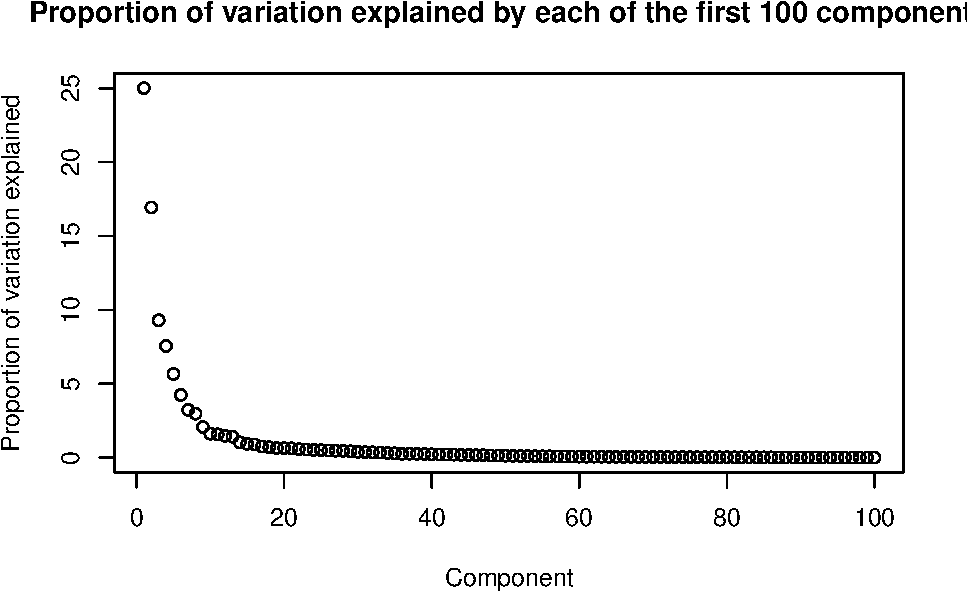
\includegraphics{Lab3_files/figure-latex/3.1-1.pdf}

\subsubsection{3.2}\label{section-1}

First of all, we define linear activation function as follows. According
to the plot, we can see that the prediction is a straight line compared
to the train and test data which shows a sine wave.

\begin{Shaded}
\begin{Highlighting}[]
\DocumentationTok{\#\#\#\#\#\#\#\#\#\#\#\#\#\#\#\#\#\#\#\#\#\#\#\#\#\#\#  3.2.1 Linear \#\#\#\#\#\#\#\#\#\#\#\#\#\#\#\#\#\#\#\#\#\#\#\#\#\#\#\#\#\#\#\#\#\#\#\#\#\#\#}

\CommentTok{\#Linear}
\NormalTok{h1 }\OtherTok{\textless{}{-}} \ControlFlowTok{function}\NormalTok{(x) \{}
\NormalTok{  x}
\NormalTok{\} }

\NormalTok{nn1 }\OtherTok{\textless{}{-}} \FunctionTok{neuralnet}\NormalTok{(}\AttributeTok{data =}\NormalTok{ train, }\AttributeTok{formula =}\NormalTok{ Sin }\SpecialCharTok{\textasciitilde{}}\NormalTok{ rand\_var, }\AttributeTok{hidden =} \FunctionTok{c}\NormalTok{(}\DecValTok{10}\NormalTok{), }\AttributeTok{act.fct =}\NormalTok{ h1)}

\CommentTok{\# Plot of the training data (black), test data (blue), and predictions (red)}
\FunctionTok{plot}\NormalTok{(train,  }\AttributeTok{col =} \StringTok{"black"}\NormalTok{, }\AttributeTok{cex=}\DecValTok{1}\NormalTok{, }\AttributeTok{main=}\StringTok{"Linear"}\NormalTok{)}
\FunctionTok{points}\NormalTok{(test, }\AttributeTok{col =} \StringTok{"blue"}\NormalTok{, }\AttributeTok{cex=}\DecValTok{1}\NormalTok{)}
\FunctionTok{points}\NormalTok{(test[,}\DecValTok{1}\NormalTok{], }\FunctionTok{predict}\NormalTok{(nn1,test), }\AttributeTok{col=}\StringTok{"red"}\NormalTok{, }\AttributeTok{cex=}\DecValTok{1}\NormalTok{)}
\FunctionTok{legend}\NormalTok{(}\AttributeTok{x =} \FloatTok{6.5}\NormalTok{, }\AttributeTok{y =} \SpecialCharTok{{-}}\FloatTok{0.6}\NormalTok{, }\AttributeTok{legend =} \FunctionTok{c}\NormalTok{(}\StringTok{"Training data"}\NormalTok{, }\StringTok{"Test data"}\NormalTok{,}
\StringTok{"Pred"}\NormalTok{), }\AttributeTok{col =} \FunctionTok{c}\NormalTok{(}\StringTok{"black"}\NormalTok{, }\StringTok{"blue"}\NormalTok{, }\StringTok{"red"}\NormalTok{), }\AttributeTok{cex =} \FloatTok{0.7}\NormalTok{,}\AttributeTok{pch =} \DecValTok{1}\NormalTok{)}
\end{Highlighting}
\end{Shaded}

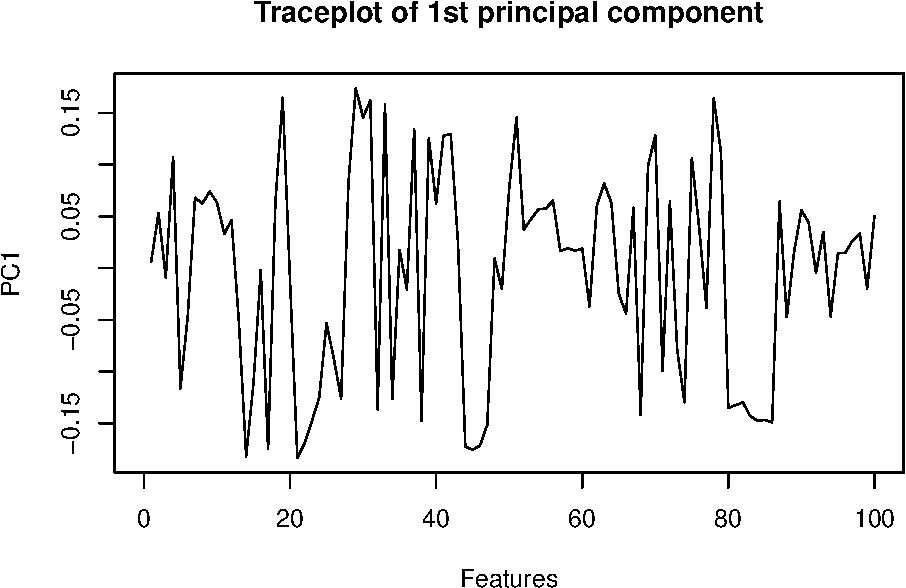
\includegraphics{Lab3_files/figure-latex/3.2.1-1.pdf}

Then we define ReLU activation function as follows, we use ifelse to
define the function since max(0,x) not working here.

As what can be seen in the plot, ReLU function as an activation function
do not provide good results on test data.

The right prediction range only in around(0.5,4) . when random variable
in range (4,10), it shows a straight line as what we see in linear
activation function.

\begin{Shaded}
\begin{Highlighting}[]
\DocumentationTok{\#\#\#\#\#\#\#\#\#\#\#\#\#\#\#\#\#\#\#\#\#\#\#\#\#\#\#  3.2.2 Relu \#\#\#\#\#\#\#\#\#\#\#\#\#\#\#\#\#\#\#\#\#\#\#\#\#\#\#\#\#\#\#\#\#\#\#\#\#\#\#}

\CommentTok{\#ReLU}
\NormalTok{h2 }\OtherTok{\textless{}{-}} \ControlFlowTok{function}\NormalTok{(x) \{}
  \CommentTok{\# max(0,x) not working}
  \FunctionTok{ifelse}\NormalTok{(x}\SpecialCharTok{\textgreater{}=}\DecValTok{0}\NormalTok{,x,}\DecValTok{0}\NormalTok{)}
\NormalTok{\}}


\NormalTok{nn2 }\OtherTok{\textless{}{-}} \FunctionTok{neuralnet}\NormalTok{(}\AttributeTok{formula =}\NormalTok{ Sin }\SpecialCharTok{\textasciitilde{}}\NormalTok{ rand\_var, }\AttributeTok{data =}\NormalTok{ train, }\AttributeTok{hidden =} \DecValTok{10}\NormalTok{,}
\AttributeTok{startweights =}\NormalTok{ winit, }\AttributeTok{act.fct =}\NormalTok{ h2)}

\CommentTok{\# Plot of the training data (black), test data (blue), and predictions (red)}
\FunctionTok{plot}\NormalTok{(train,  }\AttributeTok{col =} \StringTok{"black"}\NormalTok{, }\AttributeTok{cex=}\DecValTok{1}\NormalTok{,}\AttributeTok{main=}\StringTok{"Relu"}\NormalTok{)}
\FunctionTok{points}\NormalTok{(test, }\AttributeTok{col =} \StringTok{"blue"}\NormalTok{, }\AttributeTok{cex=}\DecValTok{1}\NormalTok{)}
\FunctionTok{points}\NormalTok{(test[,}\DecValTok{1}\NormalTok{], }\FunctionTok{predict}\NormalTok{(nn2,test), }\AttributeTok{col=}\StringTok{"red"}\NormalTok{, }\AttributeTok{cex=}\DecValTok{1}\NormalTok{)}
\FunctionTok{legend}\NormalTok{(}\AttributeTok{x =} \FloatTok{6.5}\NormalTok{, }\AttributeTok{y =} \SpecialCharTok{{-}}\FloatTok{0.6}\NormalTok{, }\AttributeTok{legend =} \FunctionTok{c}\NormalTok{(}\StringTok{"Training data"}\NormalTok{, }\StringTok{"Test data"}\NormalTok{,}
\StringTok{"Pred"}\NormalTok{), }\AttributeTok{col =} \FunctionTok{c}\NormalTok{(}\StringTok{"black"}\NormalTok{, }\StringTok{"blue"}\NormalTok{, }\StringTok{"red"}\NormalTok{), }\AttributeTok{cex =} \FloatTok{0.7}\NormalTok{,}\AttributeTok{pch =} \DecValTok{1}\NormalTok{)}
\end{Highlighting}
\end{Shaded}

\includegraphics{Lab3_files/figure-latex/3.2.2-1.pdf}

Last we define Softplus activation function as follows, as what can be
seen in the plot, Softplus function as an activation function provide
good results on test data.

\begin{Shaded}
\begin{Highlighting}[]
\DocumentationTok{\#\#\#\#\#\#\#\#\#\#\#\#\#\#\#\#\#\#\#\#\#\#\#\#\#\#\#  3.2.3 Softplus \#\#\#\#\#\#\#\#\#\#\#\#\#\#\#\#\#\#\#\#\#\#\#\#\#\#\#\#\#\#\#\#\#\#\#\#\#\#\#}

\CommentTok{\#Softplus}
\NormalTok{h3 }\OtherTok{\textless{}{-}} \ControlFlowTok{function}\NormalTok{(x) \{}
  \FunctionTok{log}\NormalTok{(}\DecValTok{1}\SpecialCharTok{+}\FunctionTok{exp}\NormalTok{(x))}
\NormalTok{\}}

\NormalTok{nn3 }\OtherTok{\textless{}{-}} \FunctionTok{neuralnet}\NormalTok{(}\AttributeTok{formula =}\NormalTok{ Sin }\SpecialCharTok{\textasciitilde{}}\NormalTok{ rand\_var, }\AttributeTok{data =}\NormalTok{ train, }\AttributeTok{hidden =} \DecValTok{10}\NormalTok{,}
\AttributeTok{startweights =}\NormalTok{ winit, }\AttributeTok{act.fct =}\NormalTok{ h3)}

\CommentTok{\# Plot of the training data (black), test data (blue), and predictions (red)}
\FunctionTok{plot}\NormalTok{(train,  }\AttributeTok{col =} \StringTok{"black"}\NormalTok{, }\AttributeTok{cex=}\DecValTok{1}\NormalTok{,}\AttributeTok{main=}\StringTok{"Softplus"}\NormalTok{)}
\FunctionTok{points}\NormalTok{(test, }\AttributeTok{col =} \StringTok{"blue"}\NormalTok{, }\AttributeTok{cex=}\DecValTok{1}\NormalTok{)}
\FunctionTok{points}\NormalTok{(test[,}\DecValTok{1}\NormalTok{], }\FunctionTok{predict}\NormalTok{(nn3,test), }\AttributeTok{col=}\StringTok{"red"}\NormalTok{, }\AttributeTok{cex=}\DecValTok{1}\NormalTok{)}
\FunctionTok{legend}\NormalTok{(}\AttributeTok{x =} \FloatTok{6.5}\NormalTok{, }\AttributeTok{y =} \SpecialCharTok{{-}}\FloatTok{0.6}\NormalTok{, }\AttributeTok{legend =} \FunctionTok{c}\NormalTok{(}\StringTok{"Training data"}\NormalTok{, }\StringTok{"Test data"}\NormalTok{,}
\StringTok{"Pred"}\NormalTok{), }\AttributeTok{col =} \FunctionTok{c}\NormalTok{(}\StringTok{"black"}\NormalTok{, }\StringTok{"blue"}\NormalTok{, }\StringTok{"red"}\NormalTok{), }\AttributeTok{cex =} \FloatTok{0.7}\NormalTok{,}\AttributeTok{pch =} \DecValTok{1}\NormalTok{)}
\end{Highlighting}
\end{Shaded}

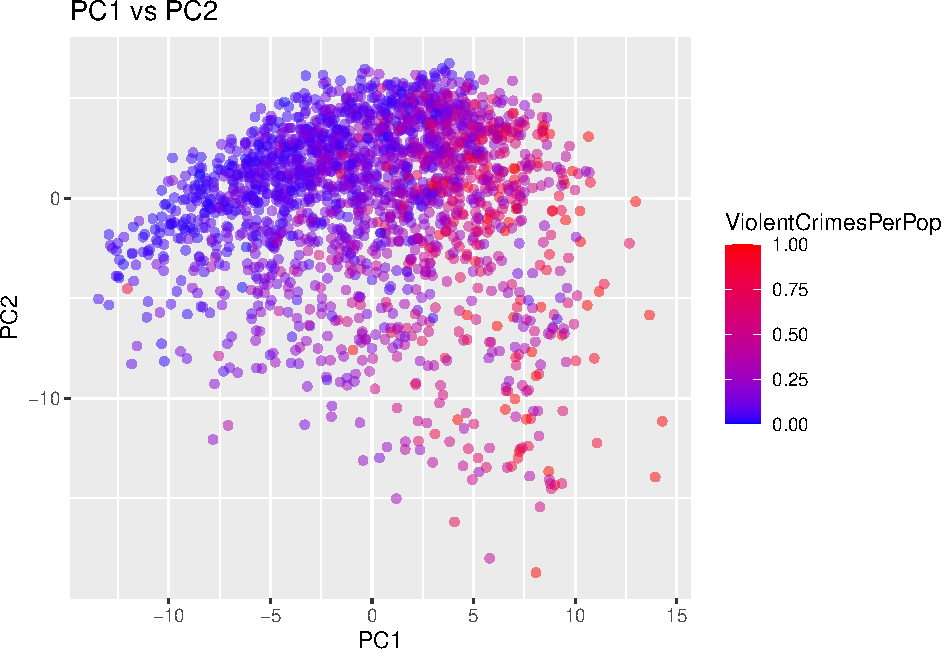
\includegraphics{Lab3_files/figure-latex/3.2.3-1.pdf}

\subsubsection{3.3}\label{section-2}

The code is as follows. When random in range (0,10), the prediction is
match the test data, when it is greater than 10, the prediction begin to
get smaller and eventually convergeing to a value which is around -3.

\begin{Shaded}
\begin{Highlighting}[]
\DocumentationTok{\#\#\#\#\#\#\#\#\#\#\#\#\#\#\#\#\#\#\#\#\#\#\#\#\#\#\#  3.3  \#\#\#\#\#\#\#\#\#\#\#\#\#\#\#\#\#\#\#\#\#\#\#\#\#\#\#\#\#\#\#\#\#\#\#\#\#\#\#}
\CommentTok{\# Sample 500 points}
\FunctionTok{set.seed}\NormalTok{(}\DecValTok{1234567890}\NormalTok{)}
\NormalTok{rand\_var }\OtherTok{\textless{}{-}} \FunctionTok{runif}\NormalTok{(}\DecValTok{500}\NormalTok{, }\AttributeTok{min =} \DecValTok{0}\NormalTok{, }\AttributeTok{max =} \DecValTok{50}\NormalTok{) }
\NormalTok{df }\OtherTok{\textless{}{-}} \FunctionTok{data.frame}\NormalTok{(rand\_var, }\AttributeTok{Sin =} \FunctionTok{sin}\NormalTok{(rand\_var))}
\FunctionTok{plot}\NormalTok{(train, }\AttributeTok{cex =} \DecValTok{2}\NormalTok{, }\AttributeTok{xlim =} \FunctionTok{c}\NormalTok{(}\DecValTok{0}\NormalTok{, }\DecValTok{50}\NormalTok{), }\AttributeTok{ylim =} \FunctionTok{c}\NormalTok{(}\SpecialCharTok{{-}}\DecValTok{6}\NormalTok{, }\DecValTok{2}\NormalTok{))}
\FunctionTok{points}\NormalTok{(df, }\AttributeTok{col =} \StringTok{"blue"}\NormalTok{, }\AttributeTok{cex =} \DecValTok{1}\NormalTok{)}
\FunctionTok{points}\NormalTok{(df[, }\DecValTok{1}\NormalTok{], }\FunctionTok{predict}\NormalTok{(nn, df), }\AttributeTok{col =} \StringTok{"red"}\NormalTok{, }\AttributeTok{cex =} \DecValTok{1}\NormalTok{)}
\end{Highlighting}
\end{Shaded}

\includegraphics{Lab3_files/figure-latex/3.3-1.pdf}

\begin{Shaded}
\begin{Highlighting}[]
\FunctionTok{plot}\NormalTok{(nn)}
\end{Highlighting}
\end{Shaded}

\subsubsection{3.4}\label{section-3}

We define the following code to get the value of the convergence. by
setting a relativ big value 100, we can calculate the approximation
value of the convergence around -3.105391.

\begin{Shaded}
\begin{Highlighting}[]
\DocumentationTok{\#\#\#\#\#\#\#\#\#\#\#\#\#\#\#\#\#\#\#\#\#\#\#\#\#\#\#  3.4  \#\#\#\#\#\#\#\#\#\#\#\#\#\#\#\#\#\#\#\#\#\#\#\#\#\#\#\#\#\#\#\#\#\#\#\#\#\#\#}

\NormalTok{sigmoid }\OtherTok{\textless{}{-}} \ControlFlowTok{function}\NormalTok{(x)\{}
  \FunctionTok{return}\NormalTok{(}\DecValTok{1} \SpecialCharTok{/}\NormalTok{ (}\DecValTok{1} \SpecialCharTok{+} \FunctionTok{exp}\NormalTok{(}\SpecialCharTok{{-}}\NormalTok{x)))}
\NormalTok{\}}
\CommentTok{\#}
\NormalTok{weight\_1 }\OtherTok{\textless{}{-}}\NormalTok{ nn}\SpecialCharTok{$}\NormalTok{weights[[}\DecValTok{1}\NormalTok{]][[}\DecValTok{1}\NormalTok{]][}\DecValTok{2}\NormalTok{,]}
\NormalTok{bias\_1 }\OtherTok{\textless{}{-}}\NormalTok{ nn}\SpecialCharTok{$}\NormalTok{weights[[}\DecValTok{1}\NormalTok{]][[}\DecValTok{1}\NormalTok{]][}\DecValTok{1}\NormalTok{,]}

\NormalTok{sigmoid\_val }\OtherTok{\textless{}{-}} \FunctionTok{sigmoid}\NormalTok{(weight\_1 }\SpecialCharTok{*} \DecValTok{100} \SpecialCharTok{+}\NormalTok{ bias\_1)}

\NormalTok{bias\_2 }\OtherTok{\textless{}{-}}\NormalTok{ nn}\SpecialCharTok{$}\NormalTok{weights[[}\DecValTok{1}\NormalTok{]][[}\DecValTok{2}\NormalTok{]][}\DecValTok{1}\NormalTok{,]}
\NormalTok{weight\_2 }\OtherTok{\textless{}{-}}\NormalTok{ nn}\SpecialCharTok{$}\NormalTok{weights[[}\DecValTok{1}\NormalTok{]][[}\DecValTok{2}\NormalTok{]][}\DecValTok{2}\SpecialCharTok{:}\DecValTok{11}\NormalTok{,]}
\FunctionTok{cat}\NormalTok{(}\StringTok{"The value will converge to:"}\NormalTok{, weight\_2 }\SpecialCharTok{\%*\%}\NormalTok{ sigmoid\_val }\SpecialCharTok{+}\NormalTok{ bias\_2, }\StringTok{"}\SpecialCharTok{\textbackslash{}n}\StringTok{"}\NormalTok{)}
\end{Highlighting}
\end{Shaded}

\begin{verbatim}
## The value will converge to: -3.105391
\end{verbatim}

\subsubsection{3.5}\label{section-4}

The code as follows.

We can see that the pridcton is not good, the reason is many input
values can be mapping to a same value if we using sine function, but if
we inverse this function, the original input value can not be calculated
through the inverse of sine function.so the NN can not learn the mapping
relationship between input and output and generate a bad prediction.

\begin{Shaded}
\begin{Highlighting}[]
\DocumentationTok{\#\#\#\#\#\#\#\#\#\#\#\#\#\#\#\#\#\#\#\#\#\#\#\#\#\#\#  3.5  \#\#\#\#\#\#\#\#\#\#\#\#\#\#\#\#\#\#\#\#\#\#\#\#\#\#\#\#\#\#\#\#\#\#\#\#\#\#\#}

\CommentTok{\# Sample 500 points}
\NormalTok{rand\_var }\OtherTok{\textless{}{-}} \FunctionTok{runif}\NormalTok{(}\DecValTok{500}\NormalTok{, }\AttributeTok{min =} \DecValTok{0}\NormalTok{, }\AttributeTok{max =} \DecValTok{10}\NormalTok{) }
\NormalTok{df }\OtherTok{\textless{}{-}} \FunctionTok{data.frame}\NormalTok{(}\AttributeTok{Sin =} \FunctionTok{sin}\NormalTok{(rand\_var), rand\_var)}
\NormalTok{nn4 }\OtherTok{\textless{}{-}} \FunctionTok{neuralnet}\NormalTok{(}\AttributeTok{formula =}\NormalTok{ rand\_var }\SpecialCharTok{\textasciitilde{}}\NormalTok{ Sin, }\AttributeTok{data =}\NormalTok{ df, }\AttributeTok{hidden =} \DecValTok{10}\NormalTok{, }\AttributeTok{startweights =}\NormalTok{ winit, }\AttributeTok{threshold =} \FloatTok{0.1}\NormalTok{)}
\NormalTok{pred\_4 }\OtherTok{\textless{}{-}} \FunctionTok{predict}\NormalTok{(nn4, df)}

\FunctionTok{plot}\NormalTok{(df, }\AttributeTok{cex =} \DecValTok{2}\NormalTok{, }\AttributeTok{col =} \StringTok{"blue"}\NormalTok{)}
\FunctionTok{points}\NormalTok{(df[, }\DecValTok{2}\NormalTok{], pred\_4, }\AttributeTok{col =} \StringTok{"red"}\NormalTok{, }\AttributeTok{cex =} \DecValTok{1}\NormalTok{)}
\FunctionTok{legend}\NormalTok{(}\AttributeTok{x =} \SpecialCharTok{{-}}\DecValTok{1}\NormalTok{, }\AttributeTok{y =} \FloatTok{8.5}\NormalTok{, }\AttributeTok{legend =} \FunctionTok{c}\NormalTok{(}\StringTok{"Training data"}\NormalTok{, }\StringTok{"NN Pred"}\NormalTok{),}
\AttributeTok{col =} \FunctionTok{c}\NormalTok{(}\StringTok{"blue"}\NormalTok{, }\StringTok{"red"}\NormalTok{), }\AttributeTok{cex =} \DecValTok{1}\NormalTok{, }\AttributeTok{pch =} \DecValTok{1}\NormalTok{)}
\end{Highlighting}
\end{Shaded}

\includegraphics{Lab3_files/figure-latex/3.5-1.pdf}

\newpage

\subsection{Appendix: All code for this
report}\label{appendix-all-code-for-this-report}

\begin{Shaded}
\begin{Highlighting}[]
\DocumentationTok{\#\#\#\#\#\#\#\#\#\#\#\#\#\#\#\#\#\#\#\#\#\#\#\#\#\#\#  Init code For Assignment 1 \#\#\#\#\#\#\#\#\#\#\#\#\#\#\#\#\#\#\#\#\#\#\#\#}
\FunctionTok{rm}\NormalTok{(}\AttributeTok{list =} \FunctionTok{ls}\NormalTok{())}
\NormalTok{knitr}\SpecialCharTok{::}\NormalTok{opts\_chunk}\SpecialCharTok{$}\FunctionTok{set}\NormalTok{(}\AttributeTok{echo =} \ConstantTok{TRUE}\NormalTok{)}
\FunctionTok{library}\NormalTok{(geosphere)}
\FunctionTok{set.seed}\NormalTok{(}\DecValTok{1234567890}\NormalTok{)}
\DocumentationTok{\#\#\#\#\#\#\#\#\#\#\#\#\#\#\#\#\#\#\#\#\#\#\#\#\#\#\#\# init data \#\#\#\#\#\#\#\#\#\#\#\#\#\#\#\#\#\#\#\#\#\#\#\#\#\#\#\#\#\#\#\#\#\#\#\#\#\#}
\NormalTok{stations }\OtherTok{\textless{}{-}} \FunctionTok{read.csv}\NormalTok{(}\StringTok{"stations.csv"}\NormalTok{, }\AttributeTok{fileEncoding =} \StringTok{"latin1"}\NormalTok{)}
\NormalTok{temps }\OtherTok{\textless{}{-}} \FunctionTok{read.csv}\NormalTok{(}\StringTok{"temps50k.csv"}\NormalTok{)}
\NormalTok{st }\OtherTok{\textless{}{-}} \FunctionTok{merge}\NormalTok{(stations, temps, }\AttributeTok{by =} \StringTok{"station\_number"}\NormalTok{)}

\CommentTok{\# define date of interest}
\NormalTok{date\_interest }\OtherTok{\textless{}{-}} \FunctionTok{as.Date}\NormalTok{(}\StringTok{"1970{-}11{-}05"}\NormalTok{)}

\CommentTok{\# filter out data which is later than data of interest }
\NormalTok{st}\SpecialCharTok{$}\NormalTok{date }\OtherTok{\textless{}{-}} \FunctionTok{as.Date}\NormalTok{(st}\SpecialCharTok{$}\NormalTok{date)}
\NormalTok{old\_sf }\OtherTok{\textless{}{-}}\NormalTok{ st }\CommentTok{\#for later use}
\NormalTok{st }\OtherTok{\textless{}{-}}\NormalTok{ st[}\SpecialCharTok{{-}}\FunctionTok{which}\NormalTok{(}\FunctionTok{difftime}\NormalTok{(date\_interest, st}\SpecialCharTok{$}\NormalTok{date) }\SpecialCharTok{\textless{}=} \DecValTok{0}\NormalTok{),]}

\CommentTok{\# define station of interest to Linköping}
\NormalTok{station\_row }\OtherTok{\textless{}{-}} \FunctionTok{which}\NormalTok{(stations}\SpecialCharTok{$}\NormalTok{station\_name }\SpecialCharTok{==} \StringTok{"Linköping"}\NormalTok{) }
\NormalTok{station }\OtherTok{\textless{}{-}}\NormalTok{ stations}\SpecialCharTok{$}\NormalTok{station\_name[station\_row] }

\CommentTok{\# split the data to train and test (70/30)}
\NormalTok{n }\OtherTok{\textless{}{-}} \FunctionTok{dim}\NormalTok{(st)[}\DecValTok{1}\NormalTok{]}
\NormalTok{id }\OtherTok{\textless{}{-}} \FunctionTok{sample}\NormalTok{(}\DecValTok{1}\SpecialCharTok{:}\NormalTok{n, }\FunctionTok{floor}\NormalTok{(n }\SpecialCharTok{*} \FloatTok{0.7}\NormalTok{))}
\NormalTok{train }\OtherTok{\textless{}{-}}\NormalTok{ st[id, ]}
\NormalTok{test }\OtherTok{\textless{}{-}}\NormalTok{ st[}\SpecialCharTok{{-}}\NormalTok{id, ]}
\DocumentationTok{\#\#\#\#\#\#\#\#\#\#\#\#\#\#\#\#\#\#\#\#\#\#\#\#\# Kernel Code  \#\#\#\#\#\#\#\#\#\#\#\#\#\#\#\#\#\#\#\#\#\#\#\#\#\#\#\#\#\#\#\#\#\#\#\#\#}
\CommentTok{\# Gaussian kernel of geo distance}
\NormalTok{geo\_distance }\OtherTok{\textless{}{-}} \ControlFlowTok{function}\NormalTok{(data, location\_interest, h\_dist) \{}
\NormalTok{  location }\OtherTok{\textless{}{-}} \FunctionTok{data.frame}\NormalTok{(}\AttributeTok{longitude =}\NormalTok{ data}\SpecialCharTok{$}\NormalTok{longitude,}
                         \AttributeTok{latitude  =}\NormalTok{ data}\SpecialCharTok{$}\NormalTok{latitude)}
\NormalTok{  distances }\OtherTok{\textless{}{-}} \FunctionTok{distHaversine}\NormalTok{(location\_interest,location)}
\NormalTok{  kernel\_result }\OtherTok{\textless{}{-}} \FunctionTok{exp}\NormalTok{(}\SpecialCharTok{{-}}\NormalTok{(distances)}\SpecialCharTok{\^{}}\DecValTok{2} \SpecialCharTok{/}\NormalTok{ (}\DecValTok{2} \SpecialCharTok{*}\NormalTok{ h\_dist}\SpecialCharTok{\^{}}\DecValTok{2}\NormalTok{))}
  \FunctionTok{return}\NormalTok{(}\FunctionTok{c}\NormalTok{(distances, kernel\_result))}
\NormalTok{\}}

\CommentTok{\# Gaussian kernel of day distance}
\NormalTok{day\_distance }\OtherTok{\textless{}{-}} \ControlFlowTok{function}\NormalTok{(data, day\_interest, h\_day) \{}
\NormalTok{  distances }\OtherTok{\textless{}{-}} \FunctionTok{as.numeric}\NormalTok{(}\FunctionTok{difftime}\NormalTok{(day\_interest,data, }
                          \AttributeTok{units =} \StringTok{"days"}\NormalTok{))}
\NormalTok{  kernel\_result }\OtherTok{\textless{}{-}} \FunctionTok{exp}\NormalTok{(}\SpecialCharTok{{-}}\NormalTok{(distances)}\SpecialCharTok{\^{}}\DecValTok{2} \SpecialCharTok{/}\NormalTok{ (}\DecValTok{2} \SpecialCharTok{*}\NormalTok{ h\_day}\SpecialCharTok{\^{}}\DecValTok{2}\NormalTok{))}
  \FunctionTok{return}\NormalTok{(}\FunctionTok{c}\NormalTok{(distances, kernel\_result))}
\NormalTok{\}}

\CommentTok{\# Gaussian kernel of hour distance}
\NormalTok{hour\_distance }\OtherTok{\textless{}{-}} \ControlFlowTok{function}\NormalTok{(data, hour\_interest, h\_hour) \{}
  
\NormalTok{  diff }\OtherTok{\textless{}{-}} \FunctionTok{sapply}\NormalTok{(}\DecValTok{1}\SpecialCharTok{:}\FunctionTok{length}\NormalTok{(hour\_interest), }\ControlFlowTok{function}\NormalTok{(x)\{}
              \FunctionTok{abs}\NormalTok{(}\FunctionTok{as.numeric}\NormalTok{(}\FunctionTok{difftime}\NormalTok{(}\FunctionTok{strptime}\NormalTok{(hour\_interest[x], }\StringTok{"\%H:\%M:\%S"}\NormalTok{), }
                                      \FunctionTok{strptime}\NormalTok{(data}\SpecialCharTok{$}\NormalTok{time, }\StringTok{"\%H:\%M:\%S"}\NormalTok{)), }\AttributeTok{units=}\StringTok{"hours"}\NormalTok{))}
\NormalTok{  \})}
  
\NormalTok{  distances }\OtherTok{\textless{}{-}} \FunctionTok{ifelse}\NormalTok{(diff }\SpecialCharTok{\textless{}=} \DecValTok{12}\NormalTok{, diff, }\DecValTok{24}\SpecialCharTok{{-}}\NormalTok{diff)}
\NormalTok{  kernel\_result }\OtherTok{\textless{}{-}} \FunctionTok{exp}\NormalTok{(}\SpecialCharTok{{-}}\NormalTok{(distances)}\SpecialCharTok{\^{}}\DecValTok{2} \SpecialCharTok{/}\NormalTok{ (}\DecValTok{2} \SpecialCharTok{*}\NormalTok{ h\_day}\SpecialCharTok{\^{}}\DecValTok{2}\NormalTok{))}
  \FunctionTok{return}\NormalTok{(kernel\_result)}
\NormalTok{\}}
\DocumentationTok{\#\#\#\#\#\#\#\#\#\#\#\#\#\#\#\#\#\#\#\#\#\#\#\#\#\#\#\#\#\#\#\# 1.1 Distance Kernel \#\#\#\#\#\#\#\#\#\#\#\#\#\#\#\#\#\#\#\#\#\#\#\#\#\#\#}

\CommentTok{\# These three values are up to the students}
\NormalTok{h\_distance }\OtherTok{\textless{}{-}} \DecValTok{100000}

\CommentTok{\# set coordinates to predict(Linköping)}
\NormalTok{a }\OtherTok{\textless{}{-}}\NormalTok{ stations}\SpecialCharTok{$}\NormalTok{longitude[station\_row]}
\NormalTok{b }\OtherTok{\textless{}{-}}\NormalTok{ stations}\SpecialCharTok{$}\NormalTok{latitude[station\_row]}

\NormalTok{N }\OtherTok{\textless{}{-}} \FunctionTok{nrow}\NormalTok{(train)}
\NormalTok{i }\OtherTok{\textless{}{-}} \DecValTok{1}\SpecialCharTok{:}\NormalTok{N}
\NormalTok{k\_distance }\OtherTok{\textless{}{-}} \FunctionTok{sapply}\NormalTok{(i, }\ControlFlowTok{function}\NormalTok{(i)\{}\FunctionTok{geo\_distance}\NormalTok{(train[i, ], }\FunctionTok{c}\NormalTok{(a, b), h\_distance)\})}
\FunctionTok{plot}\NormalTok{(k\_distance[}\DecValTok{1}\NormalTok{,], k\_distance[}\DecValTok{2}\NormalTok{,], }\AttributeTok{main =} \StringTok{"Distance Gaussian Kernel"}\NormalTok{, }\AttributeTok{xlab =} \StringTok{"Distance"}\NormalTok{, }\AttributeTok{ylab =} \StringTok{"K"}\NormalTok{)}
\DocumentationTok{\#\#\#\#\#\#\#\#\#\#\#\#\#\#\#\#\#\#\#\#\#\#\#\#\#\#\#\#\#\#\#\# 1.2 Day Kernel \#\#\#\#\#\#\#\#\#\#\#\#\#\#\#\#\#\#\#\#\#\#\#\#\#\#\#\#\#\#\#}
\NormalTok{h\_day }\OtherTok{\textless{}{-}} \DecValTok{20}
\NormalTok{k\_day }\OtherTok{\textless{}{-}} \FunctionTok{sapply}\NormalTok{(i, }\ControlFlowTok{function}\NormalTok{(i) }\FunctionTok{day\_distance}\NormalTok{(}\FunctionTok{as.Date}\NormalTok{(train}\SpecialCharTok{$}\NormalTok{date[i]), date\_interest, h\_day))}
\FunctionTok{plot}\NormalTok{(k\_day[}\DecValTok{1}\NormalTok{,], k\_day[}\DecValTok{2}\NormalTok{,], }\AttributeTok{main =} \StringTok{"Day Gaussian Kernel"}\NormalTok{, }\AttributeTok{xlab =} \StringTok{"Days"}\NormalTok{, }\AttributeTok{ylab =} \StringTok{"K"}\NormalTok{)}
\DocumentationTok{\#\#\#\#\#\#\#\#\#\#\#\#\#\#\#\#\#\#\#\#\#\#\#\#\#\#\#\#\#\#\#\# 1.3 Hour Kernel \#\#\#\#\#\#\#\#\#\#\#\#\#\#\#\#\#\#\#\#\#\#\#\#\#\#\#\#\#\#\#}

\NormalTok{h\_hour }\OtherTok{\textless{}{-}} \DecValTok{7}

\CommentTok{\# Get the time format we want}
\NormalTok{times\_interest }\OtherTok{\textless{}{-}} \FunctionTok{c}\NormalTok{(}\FunctionTok{paste0}\NormalTok{(}\StringTok{"0"}\NormalTok{,}\FunctionTok{seq}\NormalTok{(}\DecValTok{4}\NormalTok{,}\DecValTok{8}\NormalTok{,}\AttributeTok{by=}\DecValTok{2}\NormalTok{),}\StringTok{":00:00"}\NormalTok{), }\FunctionTok{paste0}\NormalTok{(}\FunctionTok{seq}\NormalTok{(}\DecValTok{10}\NormalTok{,}\DecValTok{24}\NormalTok{,}\AttributeTok{by=}\DecValTok{2}\NormalTok{),}\StringTok{":00:00"}\NormalTok{))}

\NormalTok{k\_hour }\OtherTok{\textless{}{-}} \FunctionTok{sapply}\NormalTok{(i, }\ControlFlowTok{function}\NormalTok{(i) }\FunctionTok{hour\_distance}\NormalTok{(train[i,], times\_interest, h\_hour))}
\DocumentationTok{\#\#\#\#\#\#\#\#\#\#\#\#\#\#\#\#\#\#\#\#\#\#\#\#\#\#\#\#\#\#\#\# 1.4 Sum Kernel \#\#\#\#\#\#\#\#\#\#\#\#\#\#\#\#\#\#\#\#\#\#\#\#\#\#\#\#\#\#\#}
\NormalTok{predicted\_temp\_sum }\OtherTok{\textless{}{-}} \FunctionTok{sapply}\NormalTok{(}\DecValTok{1}\SpecialCharTok{:}\FunctionTok{length}\NormalTok{(times\_interest), }\ControlFlowTok{function}\NormalTok{(x) }
        \FunctionTok{sum}\NormalTok{((k\_distance[}\DecValTok{2}\NormalTok{,] }\SpecialCharTok{+}\NormalTok{ k\_day[}\DecValTok{2}\NormalTok{,] }\SpecialCharTok{+}\NormalTok{ k\_hour[x,]) }\SpecialCharTok{*}\NormalTok{ train}\SpecialCharTok{$}\NormalTok{air\_temperature)}
        \SpecialCharTok{/} \FunctionTok{sum}\NormalTok{(k\_distance[}\DecValTok{2}\NormalTok{,], k\_day[}\DecValTok{2}\NormalTok{,], k\_hour[x,]))}

\FunctionTok{plot}\NormalTok{(}\FunctionTok{seq}\NormalTok{(}\DecValTok{4}\NormalTok{,}\DecValTok{24}\NormalTok{,}\AttributeTok{by=}\DecValTok{2}\NormalTok{),predicted\_temp\_sum, }\AttributeTok{type=}\StringTok{"l"}\NormalTok{, }
\AttributeTok{main =} \StringTok{"Temp in Linkoping(Sum)"}\NormalTok{, }\AttributeTok{xlab =} \StringTok{"Time"}\NormalTok{, }\AttributeTok{ylab =} \StringTok{"Temp"}\NormalTok{)}

\DocumentationTok{\#\#\#\#\#\#\#\#\#\#\#\#\#\#\#\#\#\#\#\#\#\#\#\#\#\#\#\#\#\#\#\# 1.5 Multi Kernel \#\#\#\#\#\#\#\#\#\#\#\#\#\#\#\#\#\#\#\#\#\#\#\#\#\#\#\#\#\#\#}
\NormalTok{predicted\_temp\_mul }\OtherTok{\textless{}{-}} \FunctionTok{sapply}\NormalTok{(}\DecValTok{1}\SpecialCharTok{:}\FunctionTok{length}\NormalTok{(times\_interest), }\ControlFlowTok{function}\NormalTok{(x) }
        \FunctionTok{sum}\NormalTok{((k\_distance[}\DecValTok{2}\NormalTok{,] }\SpecialCharTok{*}\NormalTok{ k\_day[}\DecValTok{2}\NormalTok{,] }\SpecialCharTok{*}\NormalTok{ k\_hour[x,]) }\SpecialCharTok{*}\NormalTok{ train}\SpecialCharTok{$}\NormalTok{air\_temperature)}
        \SpecialCharTok{/} \FunctionTok{sum}\NormalTok{(k\_distance[}\DecValTok{2}\NormalTok{,] }\SpecialCharTok{*}\NormalTok{ k\_day[}\DecValTok{2}\NormalTok{,] }\SpecialCharTok{*}\NormalTok{ k\_hour[x,]))}

\FunctionTok{plot}\NormalTok{(}\FunctionTok{seq}\NormalTok{(}\DecValTok{4}\NormalTok{,}\DecValTok{24}\NormalTok{,}\AttributeTok{by=}\DecValTok{2}\NormalTok{),predicted\_temp\_mul, }\AttributeTok{type=}\StringTok{"l"}\NormalTok{, }
\AttributeTok{main =} \StringTok{"Temp in Linkoping (Mul)"}\NormalTok{, }\AttributeTok{xlab =} \StringTok{"Time"}\NormalTok{, }\AttributeTok{ylab =} \StringTok{"Temp"}\NormalTok{)}



\DocumentationTok{\#\#\#\#\#\#\#\#\#\#\#\#\#\#\#\#\#\#\#\#\#\#\#\#\#\#\#  Init code For Assignment 2 \#\#\#\#\#\#\#\#\#\#\#\#\#\#\#\#\#\#\#\#\#\#\#\#}
\FunctionTok{rm}\NormalTok{(}\AttributeTok{list =} \FunctionTok{ls}\NormalTok{())}
\NormalTok{knitr}\SpecialCharTok{::}\NormalTok{opts\_chunk}\SpecialCharTok{$}\FunctionTok{set}\NormalTok{(}\AttributeTok{echo =} \ConstantTok{TRUE}\NormalTok{)}
\FunctionTok{library}\NormalTok{(kernlab)}
\FunctionTok{set.seed}\NormalTok{(}\DecValTok{1234567890}\NormalTok{)}
\DocumentationTok{\#\#\#\#\#\#\#\#\#\#\#\#\#\#\#\#\#\#\#\#\#\#\#\#\#\#\#  Load Data and split data sets \#\#\#\#\#\#\#\#\#\#\#\#\#\#\#\#\#\#\#\#\#}
\FunctionTok{data}\NormalTok{(spam)}
\NormalTok{foo }\OtherTok{\textless{}{-}} \FunctionTok{sample}\NormalTok{(}\FunctionTok{nrow}\NormalTok{(spam))}
\NormalTok{spam }\OtherTok{\textless{}{-}}\NormalTok{ spam[foo,]}
\NormalTok{spam[,}\SpecialCharTok{{-}}\DecValTok{58}\NormalTok{]}\OtherTok{\textless{}{-}}\FunctionTok{scale}\NormalTok{(spam[,}\SpecialCharTok{{-}}\DecValTok{58}\NormalTok{])}
\NormalTok{tr }\OtherTok{\textless{}{-}}\NormalTok{ spam[}\DecValTok{1}\SpecialCharTok{:}\DecValTok{3000}\NormalTok{, ]}
\NormalTok{va }\OtherTok{\textless{}{-}}\NormalTok{ spam[}\DecValTok{3001}\SpecialCharTok{:}\DecValTok{3800}\NormalTok{, ]}
\NormalTok{trva }\OtherTok{\textless{}{-}}\NormalTok{ spam[}\DecValTok{1}\SpecialCharTok{:}\DecValTok{3800}\NormalTok{, ]}
\NormalTok{te }\OtherTok{\textless{}{-}}\NormalTok{ spam[}\DecValTok{3801}\SpecialCharTok{:}\DecValTok{4601}\NormalTok{, ] }
\DocumentationTok{\#\#\#\#\#\#\#\#\#\#\#\#\#\#\#\#\#\#\#\#\#\#\#\#\#\#\#  Get error va and corresponding C \#\#\#\#\#\#\#\#\#\#\#\#\#\#\#\#\#\#\#\#\#}
\NormalTok{by }\OtherTok{\textless{}{-}} \FloatTok{0.3}
\NormalTok{err\_va }\OtherTok{\textless{}{-}} \ConstantTok{NULL}
\ControlFlowTok{for}\NormalTok{(i }\ControlFlowTok{in} \FunctionTok{seq}\NormalTok{(by,}\DecValTok{5}\NormalTok{,by))\{}
\NormalTok{  filter }\OtherTok{\textless{}{-}} \FunctionTok{ksvm}\NormalTok{(type}\SpecialCharTok{\textasciitilde{}}\NormalTok{.,}\AttributeTok{data=}\NormalTok{tr,}\AttributeTok{kernel=}\StringTok{"rbfdot"}\NormalTok{,}\AttributeTok{kpar=}\FunctionTok{list}\NormalTok{(}\AttributeTok{sigma=}\FloatTok{0.05}\NormalTok{),}\AttributeTok{C=}\NormalTok{i,}\AttributeTok{scaled=}\ConstantTok{FALSE}\NormalTok{)}
\NormalTok{  mailtype }\OtherTok{\textless{}{-}} \FunctionTok{predict}\NormalTok{(filter,va[,}\SpecialCharTok{{-}}\DecValTok{58}\NormalTok{])}
\NormalTok{  t }\OtherTok{\textless{}{-}} \FunctionTok{table}\NormalTok{(mailtype,va[,}\DecValTok{58}\NormalTok{])}
\NormalTok{  err\_va }\OtherTok{\textless{}{-}}\FunctionTok{c}\NormalTok{(err\_va,(t[}\DecValTok{1}\NormalTok{,}\DecValTok{2}\NormalTok{]}\SpecialCharTok{+}\NormalTok{t[}\DecValTok{2}\NormalTok{,}\DecValTok{1}\NormalTok{])}\SpecialCharTok{/}\FunctionTok{sum}\NormalTok{(t))}
\NormalTok{\}}

\FunctionTok{cat}\NormalTok{(}\StringTok{"minimal error ="}\NormalTok{, }\FunctionTok{min}\NormalTok{(err\_va), }\StringTok{" when C ="}\NormalTok{, }\FunctionTok{which.min}\NormalTok{(err\_va) }\SpecialCharTok{*}\NormalTok{ by,}\StringTok{"}\SpecialCharTok{\textbackslash{}n}\StringTok{"}\NormalTok{)}
\DocumentationTok{\#\#\#\#\#\#\#\#\#\#\#\#\#\#\#\#\#\#\#\#\#\#\#\#\#\#\#  Plot err\_va vs C \#\#\#\#\#\#\#\#\#\#\#\#\#\#\#\#\#\#\#\#\#}
\NormalTok{c\_plot }\OtherTok{\textless{}{-}} \FunctionTok{seq}\NormalTok{(by, }\DecValTok{5}\NormalTok{, by)}
\FunctionTok{plot}\NormalTok{(}\AttributeTok{x =}\NormalTok{ c\_plot, }\AttributeTok{y =}\NormalTok{ err\_va, }\AttributeTok{type =} \StringTok{"p"}\NormalTok{,}\AttributeTok{xlab =} \StringTok{"C"}\NormalTok{, }\AttributeTok{ylab =} \StringTok{"error\_va"}\NormalTok{, }\AttributeTok{main =} \StringTok{"err\_va vs C"}\NormalTok{)}

\NormalTok{filter0 }\OtherTok{\textless{}{-}} \FunctionTok{ksvm}\NormalTok{(type}\SpecialCharTok{\textasciitilde{}}\NormalTok{.,}\AttributeTok{data=}\NormalTok{tr,}\AttributeTok{kernel=}\StringTok{"rbfdot"}\NormalTok{,}\AttributeTok{kpar=}\FunctionTok{list}\NormalTok{(}\AttributeTok{sigma=}\FloatTok{0.05}\NormalTok{),}\AttributeTok{C=}\FunctionTok{which.min}\NormalTok{(err\_va)}\SpecialCharTok{*}\NormalTok{by,}\AttributeTok{scaled=}\ConstantTok{FALSE}\NormalTok{)}
\NormalTok{mailtype }\OtherTok{\textless{}{-}} \FunctionTok{predict}\NormalTok{(filter0,va[,}\SpecialCharTok{{-}}\DecValTok{58}\NormalTok{])}
\NormalTok{t }\OtherTok{\textless{}{-}} \FunctionTok{table}\NormalTok{(mailtype,va[,}\DecValTok{58}\NormalTok{])}
\NormalTok{err0 }\OtherTok{\textless{}{-}}\NormalTok{ (t[}\DecValTok{1}\NormalTok{,}\DecValTok{2}\NormalTok{]}\SpecialCharTok{+}\NormalTok{t[}\DecValTok{2}\NormalTok{,}\DecValTok{1}\NormalTok{])}\SpecialCharTok{/}\FunctionTok{sum}\NormalTok{(t)}

\NormalTok{filter1 }\OtherTok{\textless{}{-}} \FunctionTok{ksvm}\NormalTok{(type}\SpecialCharTok{\textasciitilde{}}\NormalTok{.,}\AttributeTok{data=}\NormalTok{tr,}\AttributeTok{kernel=}\StringTok{"rbfdot"}\NormalTok{,}\AttributeTok{kpar=}\FunctionTok{list}\NormalTok{(}\AttributeTok{sigma=}\FloatTok{0.05}\NormalTok{),}\AttributeTok{C=}\FunctionTok{which.min}\NormalTok{(err\_va)}\SpecialCharTok{*}\NormalTok{by,}\AttributeTok{scaled=}\ConstantTok{FALSE}\NormalTok{)}
\NormalTok{mailtype }\OtherTok{\textless{}{-}} \FunctionTok{predict}\NormalTok{(filter1,te[,}\SpecialCharTok{{-}}\DecValTok{58}\NormalTok{])}
\NormalTok{t }\OtherTok{\textless{}{-}} \FunctionTok{table}\NormalTok{(mailtype,te[,}\DecValTok{58}\NormalTok{])}
\NormalTok{err1 }\OtherTok{\textless{}{-}}\NormalTok{ (t[}\DecValTok{1}\NormalTok{,}\DecValTok{2}\NormalTok{]}\SpecialCharTok{+}\NormalTok{t[}\DecValTok{2}\NormalTok{,}\DecValTok{1}\NormalTok{])}\SpecialCharTok{/}\FunctionTok{sum}\NormalTok{(t)}

\NormalTok{filter2 }\OtherTok{\textless{}{-}} \FunctionTok{ksvm}\NormalTok{(type}\SpecialCharTok{\textasciitilde{}}\NormalTok{.,}\AttributeTok{data=}\NormalTok{trva,}\AttributeTok{kernel=}\StringTok{"rbfdot"}\NormalTok{,}\AttributeTok{kpar=}\FunctionTok{list}\NormalTok{(}\AttributeTok{sigma=}\FloatTok{0.05}\NormalTok{),}\AttributeTok{C=}\FunctionTok{which.min}\NormalTok{(err\_va)}\SpecialCharTok{*}\NormalTok{by,}\AttributeTok{scaled=}\ConstantTok{FALSE}\NormalTok{)}
\NormalTok{mailtype }\OtherTok{\textless{}{-}} \FunctionTok{predict}\NormalTok{(filter2,te[,}\SpecialCharTok{{-}}\DecValTok{58}\NormalTok{])}
\NormalTok{t }\OtherTok{\textless{}{-}} \FunctionTok{table}\NormalTok{(mailtype,te[,}\DecValTok{58}\NormalTok{])}
\NormalTok{err2 }\OtherTok{\textless{}{-}}\NormalTok{ (t[}\DecValTok{1}\NormalTok{,}\DecValTok{2}\NormalTok{]}\SpecialCharTok{+}\NormalTok{t[}\DecValTok{2}\NormalTok{,}\DecValTok{1}\NormalTok{])}\SpecialCharTok{/}\FunctionTok{sum}\NormalTok{(t)}


\NormalTok{filter3 }\OtherTok{\textless{}{-}} \FunctionTok{ksvm}\NormalTok{(type}\SpecialCharTok{\textasciitilde{}}\NormalTok{.,}\AttributeTok{data=}\NormalTok{spam,}\AttributeTok{kernel=}\StringTok{"rbfdot"}\NormalTok{,}\AttributeTok{kpar=}\FunctionTok{list}\NormalTok{(}\AttributeTok{sigma=}\FloatTok{0.05}\NormalTok{),}\AttributeTok{C=}\FunctionTok{which.min}\NormalTok{(err\_va)}\SpecialCharTok{*}\NormalTok{by,}\AttributeTok{scaled=}\ConstantTok{FALSE}\NormalTok{)}
\NormalTok{mailtype }\OtherTok{\textless{}{-}} \FunctionTok{predict}\NormalTok{(filter3,te[,}\SpecialCharTok{{-}}\DecValTok{58}\NormalTok{])}
\NormalTok{t }\OtherTok{\textless{}{-}} \FunctionTok{table}\NormalTok{(mailtype,te[,}\DecValTok{58}\NormalTok{])}
\NormalTok{err3 }\OtherTok{\textless{}{-}}\NormalTok{ (t[}\DecValTok{1}\NormalTok{,}\DecValTok{2}\NormalTok{]}\SpecialCharTok{+}\NormalTok{t[}\DecValTok{2}\NormalTok{,}\DecValTok{1}\NormalTok{])}\SpecialCharTok{/}\FunctionTok{sum}\NormalTok{(t)}

\CommentTok{\#cat("accuracy of filter0 is", (1{-}err0)*100,"\%\textbackslash{}n")}
\CommentTok{\#cat("accuracy of filter1 is", (1{-}err1)*100,"\%\textbackslash{}n")}
\CommentTok{\#cat("accuracy of filter2 is", (1{-}err2)*100,"\%\textbackslash{}n")}
\CommentTok{\#cat("accuracy of filter3 is", (1{-}err3)*100,"\%\textbackslash{}n")}
\NormalTok{filter0\_pred }\OtherTok{\textless{}{-}} \FunctionTok{predict}\NormalTok{(filter0, te, }\AttributeTok{type =} \StringTok{"response"}\NormalTok{)}
\NormalTok{filter0\_gerr }\OtherTok{\textless{}{-}} \FunctionTok{mean}\NormalTok{(filter0\_pred }\SpecialCharTok{!=}\NormalTok{ te[, }\DecValTok{58}\NormalTok{])}

\NormalTok{filter1\_pred }\OtherTok{\textless{}{-}} \FunctionTok{predict}\NormalTok{(filter1, te, }\AttributeTok{type =} \StringTok{"response"}\NormalTok{)}
\NormalTok{filter1\_gerr }\OtherTok{\textless{}{-}} \FunctionTok{mean}\NormalTok{(filter1\_pred }\SpecialCharTok{!=}\NormalTok{ te[, }\DecValTok{58}\NormalTok{])}

\NormalTok{filter2\_pred }\OtherTok{\textless{}{-}} \FunctionTok{predict}\NormalTok{(filter2, te, }\AttributeTok{type =} \StringTok{"response"}\NormalTok{)}
\NormalTok{filter2\_gerr }\OtherTok{\textless{}{-}} \FunctionTok{mean}\NormalTok{(filter2\_pred }\SpecialCharTok{!=}\NormalTok{ te[, }\DecValTok{58}\NormalTok{])}

\NormalTok{filter3\_pred }\OtherTok{\textless{}{-}} \FunctionTok{predict}\NormalTok{(filter3, te, }\AttributeTok{type =} \StringTok{"response"}\NormalTok{)}
\NormalTok{filter3\_gerr }\OtherTok{\textless{}{-}} \FunctionTok{mean}\NormalTok{(filter3\_pred }\SpecialCharTok{!=}\NormalTok{ te[, }\DecValTok{58}\NormalTok{])}

\FunctionTok{cat}\NormalTok{(}\StringTok{"generalization error of filter0 is"}\NormalTok{, filter0\_gerr}\SpecialCharTok{*}\DecValTok{100}\NormalTok{,}\StringTok{"\%}\SpecialCharTok{\textbackslash{}n}\StringTok{"}\NormalTok{)}
\FunctionTok{cat}\NormalTok{(}\StringTok{"generalization error of filter1 is"}\NormalTok{, filter1\_gerr}\SpecialCharTok{*}\DecValTok{100}\NormalTok{,}\StringTok{"\%}\SpecialCharTok{\textbackslash{}n}\StringTok{"}\NormalTok{)}
\FunctionTok{cat}\NormalTok{(}\StringTok{"generalization error of filter2 is"}\NormalTok{, filter2\_gerr}\SpecialCharTok{*}\DecValTok{100}\NormalTok{,}\StringTok{"\%}\SpecialCharTok{\textbackslash{}n}\StringTok{"}\NormalTok{)}
\FunctionTok{cat}\NormalTok{(}\StringTok{"generalization error of filter3 is"}\NormalTok{, filter3\_gerr}\SpecialCharTok{*}\DecValTok{100}\NormalTok{,}\StringTok{"\%}\SpecialCharTok{\textbackslash{}n}\StringTok{"}\NormalTok{)}
\NormalTok{sv }\OtherTok{\textless{}{-}} \FunctionTok{alphaindex}\NormalTok{(filter3)[[}\DecValTok{1}\NormalTok{]]}
\NormalTok{co}\OtherTok{\textless{}{-}}\FunctionTok{coef}\NormalTok{(filter3)[[}\DecValTok{1}\NormalTok{]]}
\NormalTok{inte}\OtherTok{\textless{}{-}} \SpecialCharTok{{-}} \FunctionTok{b}\NormalTok{(filter3)}
\CommentTok{\# RBF kernel with sigma = 0.05}
\NormalTok{rbf }\OtherTok{\textless{}{-}} \FunctionTok{rbfdot}\NormalTok{(}\AttributeTok{sigma =} \FloatTok{0.05}\NormalTok{) }
\NormalTok{k}\OtherTok{\textless{}{-}}\ConstantTok{NULL}
\CommentTok{\# We produce predictions for just the first 10 points in the dataset.}
\ControlFlowTok{for}\NormalTok{(i }\ControlFlowTok{in} \DecValTok{1}\SpecialCharTok{:}\DecValTok{10}\NormalTok{)\{ }
\NormalTok{  k2}\OtherTok{\textless{}{-}}\ConstantTok{NULL}
  \ControlFlowTok{for}\NormalTok{(j }\ControlFlowTok{in} \DecValTok{1}\SpecialCharTok{:}\FunctionTok{length}\NormalTok{(sv))\{}
\NormalTok{    k2 }\OtherTok{\textless{}{-}}\NormalTok{ k2 }\SpecialCharTok{+}\NormalTok{ co[j] }\SpecialCharTok{*} \FunctionTok{rbf}\NormalTok{(}\FunctionTok{as.numeric}\NormalTok{(spam[sv[j], }\SpecialCharTok{{-}}\DecValTok{58}\NormalTok{]),}
                           \FunctionTok{as.numeric}\NormalTok{(spam[i, }\SpecialCharTok{{-}}\DecValTok{58}\NormalTok{]))}
\NormalTok{  \}}
\NormalTok{  k}\OtherTok{\textless{}{-}}\FunctionTok{c}\NormalTok{(k,  k2 }\SpecialCharTok{+}\NormalTok{ inte)}
\NormalTok{\}}
\NormalTok{k}
\NormalTok{pred\_filter3 }\OtherTok{\textless{}{-}} \FunctionTok{predict}\NormalTok{(filter3,spam[}\DecValTok{1}\SpecialCharTok{:}\DecValTok{10}\NormalTok{,}\SpecialCharTok{{-}}\DecValTok{58}\NormalTok{], }\AttributeTok{type =} \StringTok{"decision"}\NormalTok{)}
\NormalTok{pred\_filter3}
\DocumentationTok{\#\#\#\#\#\#\#\#\#\#\#\#\#\#\#\#\#\#\#\#\#\#\#\#\#\#\#  Init code For Assignment 3 \#\#\#\#\#\#\#\#\#\#\#\#\#\#\#\#\#\#\#\#\#\#\#\#}
\FunctionTok{rm}\NormalTok{(}\AttributeTok{list =} \FunctionTok{ls}\NormalTok{())}
\NormalTok{knitr}\SpecialCharTok{::}\NormalTok{opts\_chunk}\SpecialCharTok{$}\FunctionTok{set}\NormalTok{(}\AttributeTok{echo =} \ConstantTok{TRUE}\NormalTok{)}
\FunctionTok{library}\NormalTok{(neuralnet)}
\FunctionTok{set.seed}\NormalTok{(}\DecValTok{1234567890}\NormalTok{)}
\DocumentationTok{\#\#\#\#\#\#\#\#\#\#\#\#\#\#\#\#\#\#\#\#\#\#\#\#\#\#\#  3.1 \#\#\#\#\#\#\#\#\#\#\#\#\#\#\#\#\#\#\#\#\#\#\#\#\#\#\#\#\#\#\#\#\#\#\#\#\#\#\#\#\#\#\#\#\#\#\#\#}
\NormalTok{rand\_var }\OtherTok{\textless{}{-}} \FunctionTok{runif}\NormalTok{(}\DecValTok{500}\NormalTok{, }\DecValTok{0}\NormalTok{, }\DecValTok{10}\NormalTok{)}
\NormalTok{df }\OtherTok{\textless{}{-}} \FunctionTok{data.frame}\NormalTok{(rand\_var, }\AttributeTok{Sin=}\FunctionTok{sin}\NormalTok{(rand\_var))}
\NormalTok{train }\OtherTok{\textless{}{-}}\NormalTok{ df[}\DecValTok{1}\SpecialCharTok{:}\DecValTok{25}\NormalTok{,] }\CommentTok{\# Training}
\NormalTok{test }\OtherTok{\textless{}{-}}\NormalTok{ df[}\DecValTok{26}\SpecialCharTok{:}\DecValTok{500}\NormalTok{,] }\CommentTok{\# Test}

\CommentTok{\# Random initialization of the weights in the interval [{-}1, 1]}
\NormalTok{winit }\OtherTok{\textless{}{-}} \FunctionTok{runif}\NormalTok{(}\DecValTok{31}\NormalTok{, }\SpecialCharTok{{-}}\DecValTok{1}\NormalTok{, }\DecValTok{1}\NormalTok{)}
\NormalTok{nn }\OtherTok{\textless{}{-}} \FunctionTok{neuralnet}\NormalTok{(}\AttributeTok{data =}\NormalTok{ train, }\AttributeTok{formula =}\NormalTok{ Sin }\SpecialCharTok{\textasciitilde{}}\NormalTok{ rand\_var, }\AttributeTok{hidden =} \FunctionTok{c}\NormalTok{(}\DecValTok{10}\NormalTok{))}

\CommentTok{\# Plot of the training data (black), test data (blue), and predictions (red)}
\FunctionTok{plot}\NormalTok{(train,  }\AttributeTok{col =} \StringTok{"black"}\NormalTok{, }\AttributeTok{cex=}\DecValTok{1}\NormalTok{, }\AttributeTok{main=}\StringTok{"Default"}\NormalTok{)}
\FunctionTok{points}\NormalTok{(test, }\AttributeTok{col =} \StringTok{"blue"}\NormalTok{, }\AttributeTok{cex=}\DecValTok{1}\NormalTok{)}
\FunctionTok{points}\NormalTok{(test[,}\DecValTok{1}\NormalTok{], }\FunctionTok{predict}\NormalTok{(nn,test), }\AttributeTok{col=}\StringTok{"red"}\NormalTok{, }\AttributeTok{cex=}\DecValTok{1}\NormalTok{)}
\FunctionTok{legend}\NormalTok{(}\AttributeTok{x =} \FloatTok{6.5}\NormalTok{, }\AttributeTok{y =} \SpecialCharTok{{-}}\FloatTok{0.6}\NormalTok{, }\AttributeTok{legend =} \FunctionTok{c}\NormalTok{(}\StringTok{"Training data"}\NormalTok{, }\StringTok{"Test data"}\NormalTok{,}
\StringTok{"Pred"}\NormalTok{), }\AttributeTok{col =} \FunctionTok{c}\NormalTok{(}\StringTok{"black"}\NormalTok{, }\StringTok{"blue"}\NormalTok{, }\StringTok{"red"}\NormalTok{), }\AttributeTok{cex =} \FloatTok{0.7}\NormalTok{,}\AttributeTok{pch =} \DecValTok{1}\NormalTok{)}
\DocumentationTok{\#\#\#\#\#\#\#\#\#\#\#\#\#\#\#\#\#\#\#\#\#\#\#\#\#\#\#  3.2.1 Linear \#\#\#\#\#\#\#\#\#\#\#\#\#\#\#\#\#\#\#\#\#\#\#\#\#\#\#\#\#\#\#\#\#\#\#\#\#\#\#}

\CommentTok{\#Linear}
\NormalTok{h1 }\OtherTok{\textless{}{-}} \ControlFlowTok{function}\NormalTok{(x) \{}
\NormalTok{  x}
\NormalTok{\} }

\NormalTok{nn1 }\OtherTok{\textless{}{-}} \FunctionTok{neuralnet}\NormalTok{(}\AttributeTok{data =}\NormalTok{ train, }\AttributeTok{formula =}\NormalTok{ Sin }\SpecialCharTok{\textasciitilde{}}\NormalTok{ rand\_var, }\AttributeTok{hidden =} \FunctionTok{c}\NormalTok{(}\DecValTok{10}\NormalTok{), }\AttributeTok{act.fct =}\NormalTok{ h1)}

\CommentTok{\# Plot of the training data (black), test data (blue), and predictions (red)}
\FunctionTok{plot}\NormalTok{(train,  }\AttributeTok{col =} \StringTok{"black"}\NormalTok{, }\AttributeTok{cex=}\DecValTok{1}\NormalTok{, }\AttributeTok{main=}\StringTok{"Linear"}\NormalTok{)}
\FunctionTok{points}\NormalTok{(test, }\AttributeTok{col =} \StringTok{"blue"}\NormalTok{, }\AttributeTok{cex=}\DecValTok{1}\NormalTok{)}
\FunctionTok{points}\NormalTok{(test[,}\DecValTok{1}\NormalTok{], }\FunctionTok{predict}\NormalTok{(nn1,test), }\AttributeTok{col=}\StringTok{"red"}\NormalTok{, }\AttributeTok{cex=}\DecValTok{1}\NormalTok{)}
\FunctionTok{legend}\NormalTok{(}\AttributeTok{x =} \FloatTok{6.5}\NormalTok{, }\AttributeTok{y =} \SpecialCharTok{{-}}\FloatTok{0.6}\NormalTok{, }\AttributeTok{legend =} \FunctionTok{c}\NormalTok{(}\StringTok{"Training data"}\NormalTok{, }\StringTok{"Test data"}\NormalTok{,}
\StringTok{"Pred"}\NormalTok{), }\AttributeTok{col =} \FunctionTok{c}\NormalTok{(}\StringTok{"black"}\NormalTok{, }\StringTok{"blue"}\NormalTok{, }\StringTok{"red"}\NormalTok{), }\AttributeTok{cex =} \FloatTok{0.7}\NormalTok{,}\AttributeTok{pch =} \DecValTok{1}\NormalTok{)}

\DocumentationTok{\#\#\#\#\#\#\#\#\#\#\#\#\#\#\#\#\#\#\#\#\#\#\#\#\#\#\#  3.2.2 Relu \#\#\#\#\#\#\#\#\#\#\#\#\#\#\#\#\#\#\#\#\#\#\#\#\#\#\#\#\#\#\#\#\#\#\#\#\#\#\#}

\CommentTok{\#ReLU}
\NormalTok{h2 }\OtherTok{\textless{}{-}} \ControlFlowTok{function}\NormalTok{(x) \{}
  \CommentTok{\# max(0,x) not working}
  \FunctionTok{ifelse}\NormalTok{(x}\SpecialCharTok{\textgreater{}=}\DecValTok{0}\NormalTok{,x,}\DecValTok{0}\NormalTok{)}
\NormalTok{\}}


\NormalTok{nn2 }\OtherTok{\textless{}{-}} \FunctionTok{neuralnet}\NormalTok{(}\AttributeTok{formula =}\NormalTok{ Sin }\SpecialCharTok{\textasciitilde{}}\NormalTok{ rand\_var, }\AttributeTok{data =}\NormalTok{ train, }\AttributeTok{hidden =} \DecValTok{10}\NormalTok{,}
\AttributeTok{startweights =}\NormalTok{ winit, }\AttributeTok{act.fct =}\NormalTok{ h2)}

\CommentTok{\# Plot of the training data (black), test data (blue), and predictions (red)}
\FunctionTok{plot}\NormalTok{(train,  }\AttributeTok{col =} \StringTok{"black"}\NormalTok{, }\AttributeTok{cex=}\DecValTok{1}\NormalTok{,}\AttributeTok{main=}\StringTok{"Relu"}\NormalTok{)}
\FunctionTok{points}\NormalTok{(test, }\AttributeTok{col =} \StringTok{"blue"}\NormalTok{, }\AttributeTok{cex=}\DecValTok{1}\NormalTok{)}
\FunctionTok{points}\NormalTok{(test[,}\DecValTok{1}\NormalTok{], }\FunctionTok{predict}\NormalTok{(nn2,test), }\AttributeTok{col=}\StringTok{"red"}\NormalTok{, }\AttributeTok{cex=}\DecValTok{1}\NormalTok{)}
\FunctionTok{legend}\NormalTok{(}\AttributeTok{x =} \FloatTok{6.5}\NormalTok{, }\AttributeTok{y =} \SpecialCharTok{{-}}\FloatTok{0.6}\NormalTok{, }\AttributeTok{legend =} \FunctionTok{c}\NormalTok{(}\StringTok{"Training data"}\NormalTok{, }\StringTok{"Test data"}\NormalTok{,}
\StringTok{"Pred"}\NormalTok{), }\AttributeTok{col =} \FunctionTok{c}\NormalTok{(}\StringTok{"black"}\NormalTok{, }\StringTok{"blue"}\NormalTok{, }\StringTok{"red"}\NormalTok{), }\AttributeTok{cex =} \FloatTok{0.7}\NormalTok{,}\AttributeTok{pch =} \DecValTok{1}\NormalTok{)}

\DocumentationTok{\#\#\#\#\#\#\#\#\#\#\#\#\#\#\#\#\#\#\#\#\#\#\#\#\#\#\#  3.2.3 Softplus \#\#\#\#\#\#\#\#\#\#\#\#\#\#\#\#\#\#\#\#\#\#\#\#\#\#\#\#\#\#\#\#\#\#\#\#\#\#\#}

\CommentTok{\#Softplus}
\NormalTok{h3 }\OtherTok{\textless{}{-}} \ControlFlowTok{function}\NormalTok{(x) \{}
  \FunctionTok{log}\NormalTok{(}\DecValTok{1}\SpecialCharTok{+}\FunctionTok{exp}\NormalTok{(x))}
\NormalTok{\}}

\NormalTok{nn3 }\OtherTok{\textless{}{-}} \FunctionTok{neuralnet}\NormalTok{(}\AttributeTok{formula =}\NormalTok{ Sin }\SpecialCharTok{\textasciitilde{}}\NormalTok{ rand\_var, }\AttributeTok{data =}\NormalTok{ train, }\AttributeTok{hidden =} \DecValTok{10}\NormalTok{,}
\AttributeTok{startweights =}\NormalTok{ winit, }\AttributeTok{act.fct =}\NormalTok{ h3)}

\CommentTok{\# Plot of the training data (black), test data (blue), and predictions (red)}
\FunctionTok{plot}\NormalTok{(train,  }\AttributeTok{col =} \StringTok{"black"}\NormalTok{, }\AttributeTok{cex=}\DecValTok{1}\NormalTok{,}\AttributeTok{main=}\StringTok{"Softplus"}\NormalTok{)}
\FunctionTok{points}\NormalTok{(test, }\AttributeTok{col =} \StringTok{"blue"}\NormalTok{, }\AttributeTok{cex=}\DecValTok{1}\NormalTok{)}
\FunctionTok{points}\NormalTok{(test[,}\DecValTok{1}\NormalTok{], }\FunctionTok{predict}\NormalTok{(nn3,test), }\AttributeTok{col=}\StringTok{"red"}\NormalTok{, }\AttributeTok{cex=}\DecValTok{1}\NormalTok{)}
\FunctionTok{legend}\NormalTok{(}\AttributeTok{x =} \FloatTok{6.5}\NormalTok{, }\AttributeTok{y =} \SpecialCharTok{{-}}\FloatTok{0.6}\NormalTok{, }\AttributeTok{legend =} \FunctionTok{c}\NormalTok{(}\StringTok{"Training data"}\NormalTok{, }\StringTok{"Test data"}\NormalTok{,}
\StringTok{"Pred"}\NormalTok{), }\AttributeTok{col =} \FunctionTok{c}\NormalTok{(}\StringTok{"black"}\NormalTok{, }\StringTok{"blue"}\NormalTok{, }\StringTok{"red"}\NormalTok{), }\AttributeTok{cex =} \FloatTok{0.7}\NormalTok{,}\AttributeTok{pch =} \DecValTok{1}\NormalTok{)}

\DocumentationTok{\#\#\#\#\#\#\#\#\#\#\#\#\#\#\#\#\#\#\#\#\#\#\#\#\#\#\#  3.3  \#\#\#\#\#\#\#\#\#\#\#\#\#\#\#\#\#\#\#\#\#\#\#\#\#\#\#\#\#\#\#\#\#\#\#\#\#\#\#}
\CommentTok{\# Sample 500 points}
\FunctionTok{set.seed}\NormalTok{(}\DecValTok{1234567890}\NormalTok{)}
\NormalTok{rand\_var }\OtherTok{\textless{}{-}} \FunctionTok{runif}\NormalTok{(}\DecValTok{500}\NormalTok{, }\AttributeTok{min =} \DecValTok{0}\NormalTok{, }\AttributeTok{max =} \DecValTok{50}\NormalTok{) }
\NormalTok{df }\OtherTok{\textless{}{-}} \FunctionTok{data.frame}\NormalTok{(rand\_var, }\AttributeTok{Sin =} \FunctionTok{sin}\NormalTok{(rand\_var))}
\FunctionTok{plot}\NormalTok{(train, }\AttributeTok{cex =} \DecValTok{2}\NormalTok{, }\AttributeTok{xlim =} \FunctionTok{c}\NormalTok{(}\DecValTok{0}\NormalTok{, }\DecValTok{50}\NormalTok{), }\AttributeTok{ylim =} \FunctionTok{c}\NormalTok{(}\SpecialCharTok{{-}}\DecValTok{6}\NormalTok{, }\DecValTok{2}\NormalTok{))}
\FunctionTok{points}\NormalTok{(df, }\AttributeTok{col =} \StringTok{"blue"}\NormalTok{, }\AttributeTok{cex =} \DecValTok{1}\NormalTok{)}
\FunctionTok{points}\NormalTok{(df[, }\DecValTok{1}\NormalTok{], }\FunctionTok{predict}\NormalTok{(nn, df), }\AttributeTok{col =} \StringTok{"red"}\NormalTok{, }\AttributeTok{cex =} \DecValTok{1}\NormalTok{)}
\FunctionTok{plot}\NormalTok{(nn)}
\DocumentationTok{\#\#\#\#\#\#\#\#\#\#\#\#\#\#\#\#\#\#\#\#\#\#\#\#\#\#\#  3.4  \#\#\#\#\#\#\#\#\#\#\#\#\#\#\#\#\#\#\#\#\#\#\#\#\#\#\#\#\#\#\#\#\#\#\#\#\#\#\#}

\NormalTok{sigmoid }\OtherTok{\textless{}{-}} \ControlFlowTok{function}\NormalTok{(x)\{}
  \FunctionTok{return}\NormalTok{(}\DecValTok{1} \SpecialCharTok{/}\NormalTok{ (}\DecValTok{1} \SpecialCharTok{+} \FunctionTok{exp}\NormalTok{(}\SpecialCharTok{{-}}\NormalTok{x)))}
\NormalTok{\}}
\CommentTok{\#}
\NormalTok{weight\_1 }\OtherTok{\textless{}{-}}\NormalTok{ nn}\SpecialCharTok{$}\NormalTok{weights[[}\DecValTok{1}\NormalTok{]][[}\DecValTok{1}\NormalTok{]][}\DecValTok{2}\NormalTok{,]}
\NormalTok{bias\_1 }\OtherTok{\textless{}{-}}\NormalTok{ nn}\SpecialCharTok{$}\NormalTok{weights[[}\DecValTok{1}\NormalTok{]][[}\DecValTok{1}\NormalTok{]][}\DecValTok{1}\NormalTok{,]}

\NormalTok{sigmoid\_val }\OtherTok{\textless{}{-}} \FunctionTok{sigmoid}\NormalTok{(weight\_1 }\SpecialCharTok{*} \DecValTok{100} \SpecialCharTok{+}\NormalTok{ bias\_1)}

\NormalTok{bias\_2 }\OtherTok{\textless{}{-}}\NormalTok{ nn}\SpecialCharTok{$}\NormalTok{weights[[}\DecValTok{1}\NormalTok{]][[}\DecValTok{2}\NormalTok{]][}\DecValTok{1}\NormalTok{,]}
\NormalTok{weight\_2 }\OtherTok{\textless{}{-}}\NormalTok{ nn}\SpecialCharTok{$}\NormalTok{weights[[}\DecValTok{1}\NormalTok{]][[}\DecValTok{2}\NormalTok{]][}\DecValTok{2}\SpecialCharTok{:}\DecValTok{11}\NormalTok{,]}
\FunctionTok{cat}\NormalTok{(}\StringTok{"The value will converge to:"}\NormalTok{, weight\_2 }\SpecialCharTok{\%*\%}\NormalTok{ sigmoid\_val }\SpecialCharTok{+}\NormalTok{ bias\_2, }\StringTok{"}\SpecialCharTok{\textbackslash{}n}\StringTok{"}\NormalTok{)}

\DocumentationTok{\#\#\#\#\#\#\#\#\#\#\#\#\#\#\#\#\#\#\#\#\#\#\#\#\#\#\#  3.5  \#\#\#\#\#\#\#\#\#\#\#\#\#\#\#\#\#\#\#\#\#\#\#\#\#\#\#\#\#\#\#\#\#\#\#\#\#\#\#}

\CommentTok{\# Sample 500 points}
\NormalTok{rand\_var }\OtherTok{\textless{}{-}} \FunctionTok{runif}\NormalTok{(}\DecValTok{500}\NormalTok{, }\AttributeTok{min =} \DecValTok{0}\NormalTok{, }\AttributeTok{max =} \DecValTok{10}\NormalTok{) }
\NormalTok{df }\OtherTok{\textless{}{-}} \FunctionTok{data.frame}\NormalTok{(}\AttributeTok{Sin =} \FunctionTok{sin}\NormalTok{(rand\_var), rand\_var)}
\NormalTok{nn4 }\OtherTok{\textless{}{-}} \FunctionTok{neuralnet}\NormalTok{(}\AttributeTok{formula =}\NormalTok{ rand\_var }\SpecialCharTok{\textasciitilde{}}\NormalTok{ Sin, }\AttributeTok{data =}\NormalTok{ df, }\AttributeTok{hidden =} \DecValTok{10}\NormalTok{, }\AttributeTok{startweights =}\NormalTok{ winit, }\AttributeTok{threshold =} \FloatTok{0.1}\NormalTok{)}
\NormalTok{pred\_4 }\OtherTok{\textless{}{-}} \FunctionTok{predict}\NormalTok{(nn4, df)}

\FunctionTok{plot}\NormalTok{(df, }\AttributeTok{cex =} \DecValTok{2}\NormalTok{, }\AttributeTok{col =} \StringTok{"blue"}\NormalTok{)}
\FunctionTok{points}\NormalTok{(df[, }\DecValTok{2}\NormalTok{], pred\_4, }\AttributeTok{col =} \StringTok{"red"}\NormalTok{, }\AttributeTok{cex =} \DecValTok{1}\NormalTok{)}
\FunctionTok{legend}\NormalTok{(}\AttributeTok{x =} \SpecialCharTok{{-}}\DecValTok{1}\NormalTok{, }\AttributeTok{y =} \FloatTok{8.5}\NormalTok{, }\AttributeTok{legend =} \FunctionTok{c}\NormalTok{(}\StringTok{"Training data"}\NormalTok{, }\StringTok{"NN Pred"}\NormalTok{),}
\AttributeTok{col =} \FunctionTok{c}\NormalTok{(}\StringTok{"blue"}\NormalTok{, }\StringTok{"red"}\NormalTok{), }\AttributeTok{cex =} \DecValTok{1}\NormalTok{, }\AttributeTok{pch =} \DecValTok{1}\NormalTok{)}
\end{Highlighting}
\end{Shaded}


\end{document}
